\chapter{Implementierung}\label{ch:implementation}

Die Implementierung dieser Arbeit besteht aus zwei weitgehend getrennten Projekten, die jedoch miteinander kommunizieren und integriert sind.
Abschnitt~\ref{sec:expanding-fulib.org} beschreibt zunächst die Änderung, die an der Webanwendung fulib.org durchgeführt wurden.
Das dabei entstandene Werkzeug ist bis auf wenige Ausnahmen autonom für die Bewertung von Abgaben einsetzbar.
Als Erweiterung oder zusätzliches Hilfsmittel dient die \ac{vsc}-Erweiterung fulibFeedback, die in Abschnitt~\ref{sec:fulibFeedback} erläutert wird.
Insbesondere kann diese Bewertende bei der Bewertung und Studierende bei der Berichtigung von Quellcode unterstützen.
Ohne fulibFeedback sind die Bewertungsmechanismen von fulib.org unabhängig vom Quellcode nutzbar.

In diesem Kapitel wird die Hausaufgabe 3\footnote{
    \url{https://seblog.cs.uni-kassel.de/wp-content/uploads/2021/11/PM2022_Hausaufgabe03.pdf}
} aus der Veranstaltung Programmieren und Modellieren im Wintersemester 2021/22 an der Universität Kassel als laufendes Beispiel verwendet.
Die Lernziele der Hausaufgabe waren die Übersetzung eines Klassendiagramms in Java-Code, die damit verbundene Implementierung von Referenzieller Integrität\footnote{
    Dies bezeichnet ein Verhalten, bei dem durch Assoziationen verknüpfte Objekte stets in beide Richtungen konsistent verlinkt sind.
}, sowie das korrekte Testen des dabei entstehenden Programmcodes.
Diese Hausaufgabe wurde gewählt, da sie sowohl individuellen als auch schematischen Code von Studierenden erwartet.
Zudem handelt es sich um eine Hausaufgabe aus der Anfangsphase der Veranstaltung.
In dieser ist mit einer höheren Abgabenanzahl und -Vielfalt bei gleichzeitig geringerer Schwierigkeit und Komplexität im Vergleich zu späteren Aufgaben zu rechnen.

\section{Erweiterung von fulib.org}\label{sec:expanding-fulib.org}

Wesentlicher Teil der Implementierung ist die Erweiterung von fulib.org durch Hinzufügen neuer und Anpassung alter Funktionalität.
In Abschnitt~\ref{subsec:fulib.org} wurde bereits die Modulaufteilung und der Stand vor Beginn dieser Arbeit beschrieben.
Nachfolgend wird ein detaillierter Ablauf erläutert, der für die Bewertung von Hausaufgaben notwendig ist.
Dieser beginnt mit dem Erstellen von Assignments in Abschnitt~\ref{subsec:creating-assignments}.
Daraufhin werden in Abschnitt~\ref{subsec:grading} die Schritte beschrieben, die bei der Bewertung getätigt werden.
Abschnitt~\ref{subsec:statistics} zeigt, wie mithilfe der Statistiken eine Einsicht in die numerischen Hintergründe eines Assignments geboten wird.
Zuletzt wird die sogenannte Code Search-Technologie vorgestellt, die eine Suchmaschine für Quellcode in Abgaben bereitstellt.
Dies ist Inhalt von Abschnitt~\ref{subsec:code-search}.

\subsection{Erstellen von Assignments}\label{subsec:creating-assignments}

Die Benutzung von fulib.org als Werkzeug zum Bewerten von Hausaufgaben erfordert zunächst einige Vorbereitungsmaßnahmen.
Diese bestehen primär aus der Erstellung eines Assignments, das die Rahmendaten und Teilaufgaben der Hausaufgabe anders als das Hausaufgabenblatt in einem maschinenverarbeitbaren Format speichert.
Die Erstellung des Assignments verläuft über ein mehrteiliges Formular, das nachfolgend betrachtet wird.
In~\cite{bachelor-thesis} wurde bereits ein ähnlicher Ablauf beschrieben, es wurde jedoch für diese Arbeit eine Neugestaltung vorgenommen, um die wachsenden Anforderungen sinnvoll unterzubringen.

\begin{figure}
    \centering
    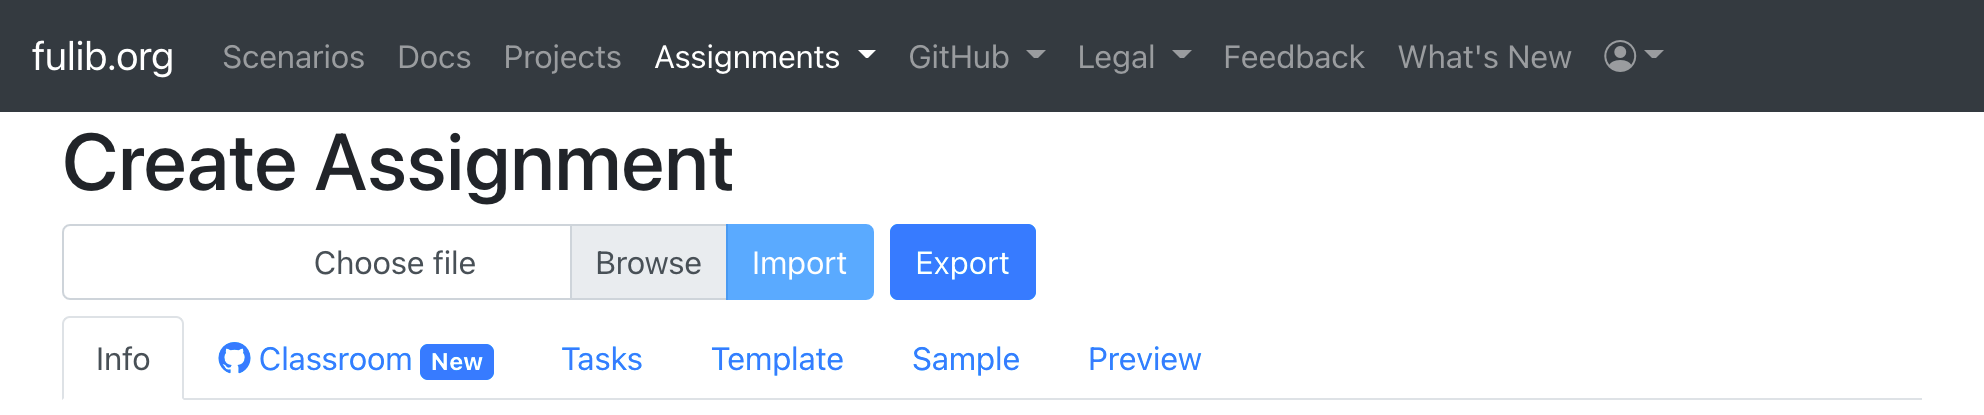
\includegraphics[width=\textwidth]{images/assignment-create-head}
    \caption{Kopf des Formulars zum Erstellen von Assignments}
    \label{fig:assignment-create-head}
\end{figure}

Abbildung~\ref{fig:assignment-create-head} stellt den Kopf des Formulars da, der stets sichtbar ist.
Hier ist es zunächst möglich, ein Assignment während der Bearbeitung zu in Form einer \ac{json}-Datei zu Exportieren oder eine solche zu Importieren.
Dies kann zur Datensicherung oder -übermittlung eingesetzt werden.
Das manuelle Speichern eines sich in Bearbeitung befindenden Assignments ist generell nicht notwendig, da nach jedem Bearbeitungsschritt sämtliche Eingaben im Browserspeicher abgelegt werden.
Dies verhindert den Datenverlust beim Unterbrechen der Bearbeitung durch Schließen des Browsertabs oder Verbindungsabbruch.
Verschiedene Registerkarten stellen die Aspekte dar, aus denen ein Assignment besteht.
Gleichzeitig ergibt sich aus ihnen eine logische Bearbeitungsreihenfolge der Schritte, in die sich der Erstellungsprozess unterteilt.
Nachfolgend werden einige dieser Aspekte und Schritte beschrieben.

\begin{figure}
    \centering
    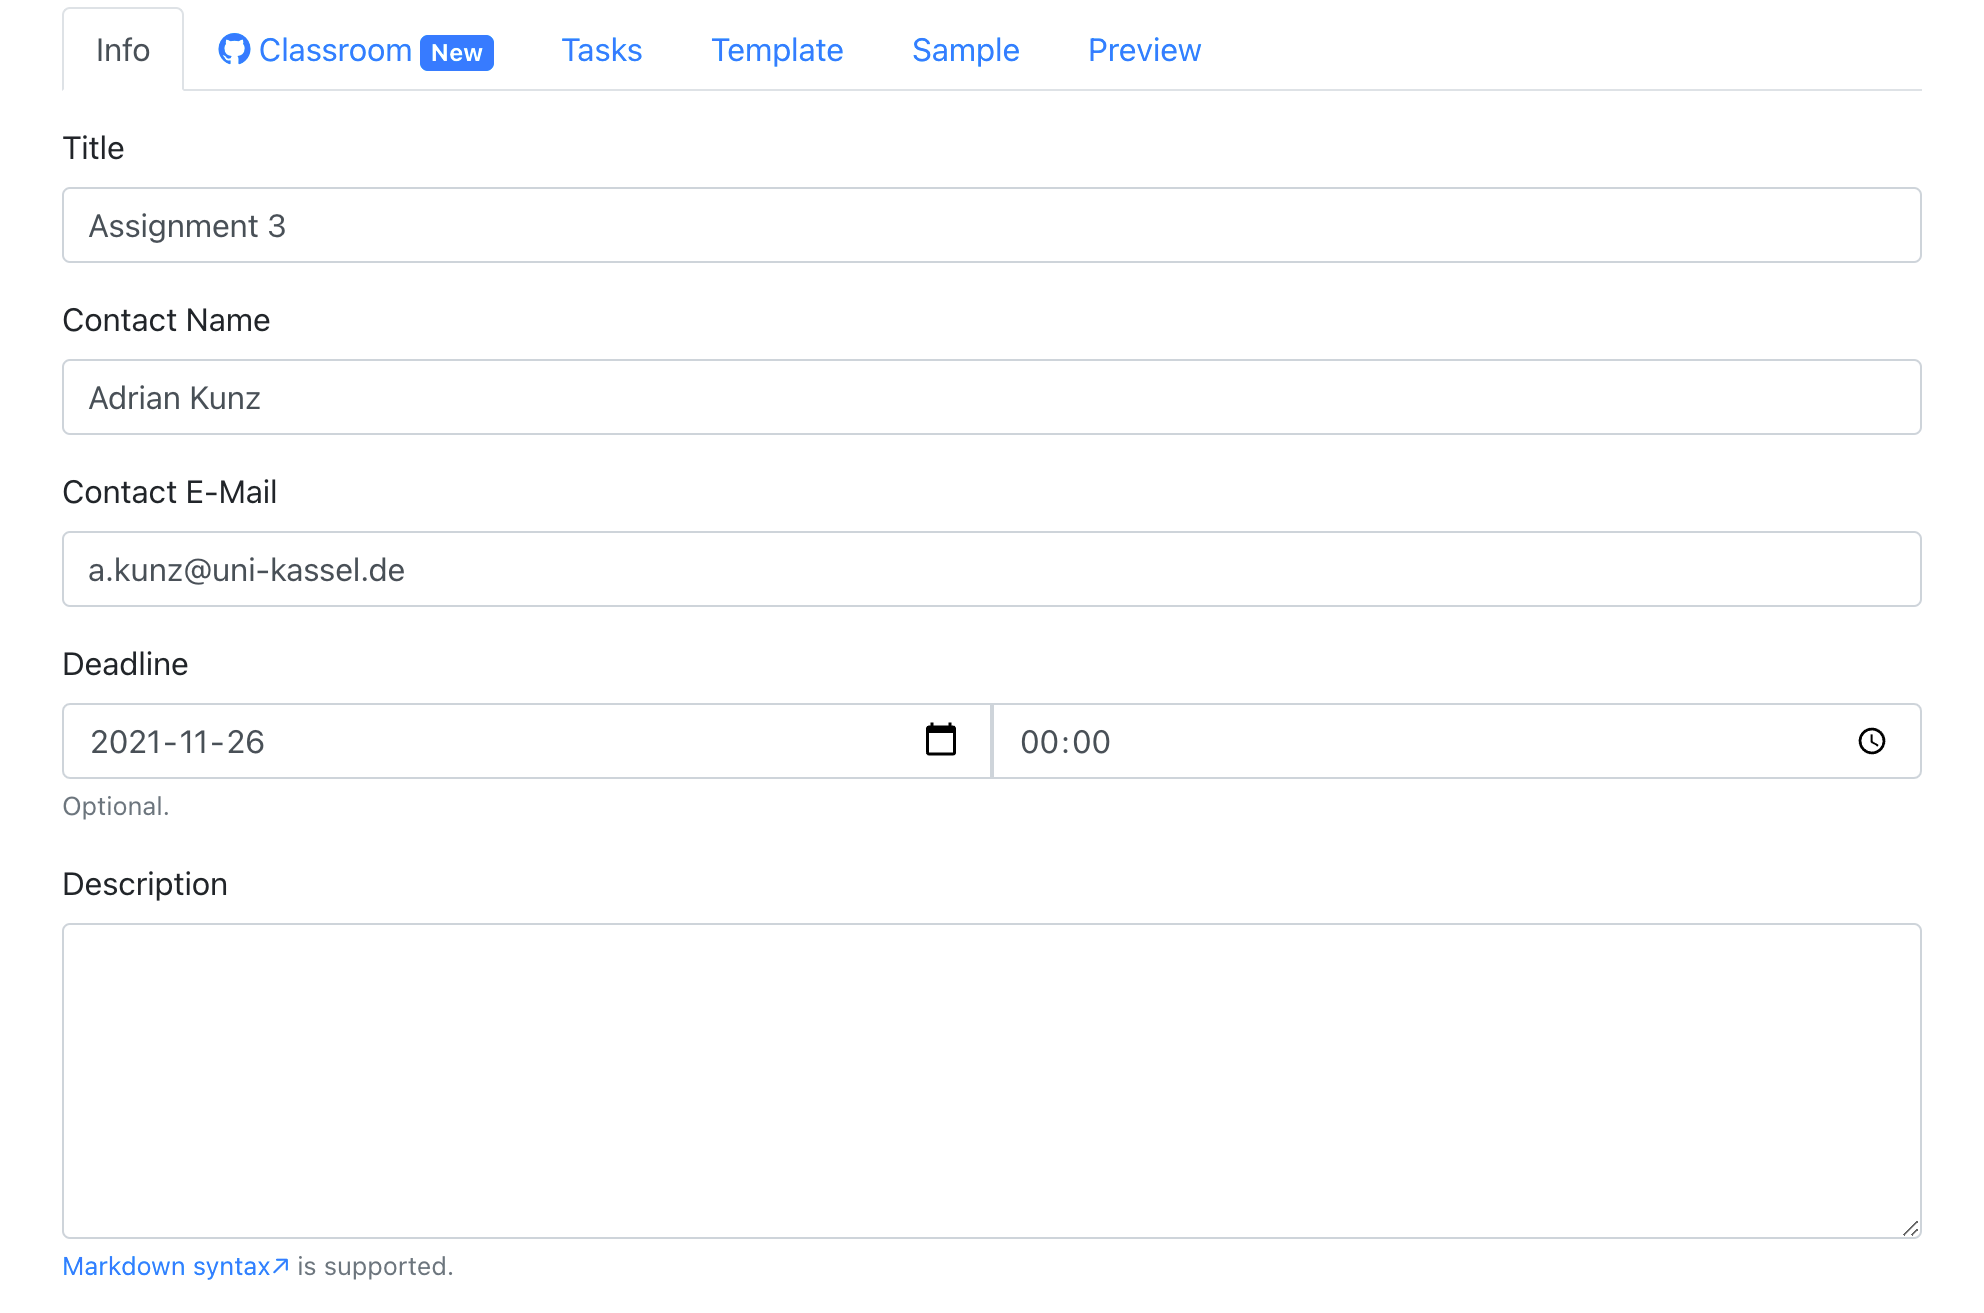
\includegraphics[width=\textwidth]{images/assignment-create-info}
    \caption{Formular für Rahmeninformationen eines Assignments}
    \label{fig:assignment-create-info}
\end{figure}

Zunächst werden einige Rahmeninformationen definiert.
Abbildung~\ref{fig:assignment-create-info} zeigt das zugehörige Formular.
Dazu gehören ein Titel (\textbf{Title}) für das Assignment, welcher der Zuordnung dient.
Ein Ansprechpartner, beispielsweise die Übungsleitung, und dessen Email-Adresse werden in den Feldern \textbf{Contact Name} und \textbf{Contact Email} festgelegt.
Die optionale Abgabefrist (\textbf{Deadline}) hat zwei wesentliche Verwendungszwecke.
Einerseits wird diese für den automatischen Import verwendet, der in Kürze anhand der GitHub Classroom-Integration erläutert wird.
Andererseits kann anhand der Deadline dargestellt werden, welche Lösungen zu spät eingereicht wurden.
Ein Beispiel dafür wird in Abschnitt~\ref{subsec:grading} gezeigt.
Die Beschreibung (\textbf{Description}) kann weitere Informationen über das Assignment enthalten, wird aber nachfolgend nicht verwendet.

\begin{figure}
    \centering
    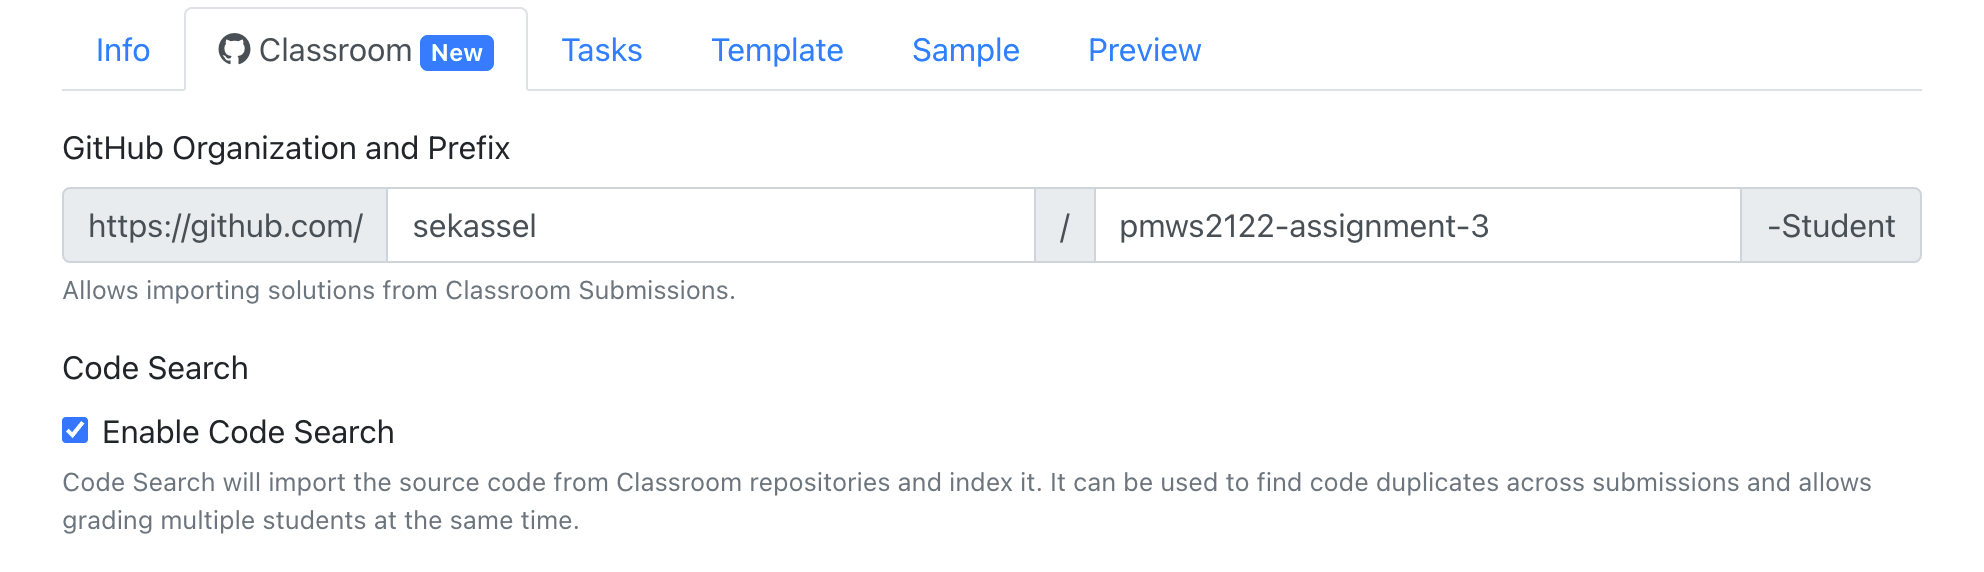
\includegraphics[width=\textwidth]{images/assignment-create-classroom}
    \caption{Formular für GitHub Classroom-Einstellungen eines Assignments}
    \label{fig:assignment-create-classroom}
\end{figure}

Auf der nächsten Seite des Formulars können Angaben für die Integration von GitHub Classroom gemacht werden.
Abbildung~\ref{fig:assignment-create-classroom} zeigt ein Bild dieses Formulars.
Dafür müssen der Name der GitHub-Organisation (\textbf{Organization}) und das Präfix (\textbf{Prefix}) konfiguriert werden.
Dies ermöglicht die manuelle oder zum Zeitpunkt der Deadline automatische Importierung von Lösungen von der Platform.
Anhand der Search-\ac{api} von GitHub\footnote{
    \url{https://docs.github.com/en/rest/reference/search\#search-repositories}
} wird nach allen Repositories in der angegebenen Organisation gesucht, deren Name mit dem Präfix beginnt.
Damit private Repositories in der Organisation gefunden werden können, muss das \textbf{GitHub Token} angegeben werden.
Der Hilfetext des Eingabefelds gibt Auskunft darüber, wie dieses erstellt werden kann.
Aus dem Repository-Name ohne Präfix kann der GitHub-Benutzername des Studierenden ermittelt werden, der für die Zuordnung der Lösung verwendet wird.
In Abschnitt~\ref{subsec:grading} ist ein Beispiel für die entstehende Lösungstabelle sichtbar.
Weiterhin wird das neueste Commit zum Zeitpunkt des Imports gespeichert, um die Reproduzierbarkeit einer Bewertung zu gewährleisten.
Insbesondere wird dadurch sichergestellt, dass Studierende ihre Lösungen nicht verfälschen, indem sie Änderungen am Quellcode nach Ablauf der Abgabefrist durchführen oder hochladen.
Anhand des Commits kann der exakte Stand zum Zeitpunkt der Abgabefrist wiederhergestellt werden.
Ist der Haken \textbf{Code Search} gesetzt, werden neben dem Commit auch die Dateien des Repositories heruntergeladen und separat gespeichert.
Diese dienen nicht der Reproduzierbarkeit, sondern der Textsuche, wie in Abschnitt~\ref{subsec:code-search} näher erläutert wird.
Aus diesem Grund wird auch kein Anspruch auf Vollständigkeit der Daten gestellt.
Vergleichsweise große Dateien (> \SI{64}{\kibi\byte}) werden nicht gespeichert, da gewöhnliche Quellcode-Dateien aus Hausaufgaben-Lösungen diese Größe nicht überschreiten.\footnote{
    Die Suche nach Quelltext-Dateien größer als \SI{64}{\kibi\byte} in der GitHub-Organisation "sekassel" ergab lediglich Ergebnisse aus Node.js-Projekten, darunter primär \code{package-lock.json}-Dateien und Dateien in versehentlich gepushten \code{node_modules}-Ordnern.
    Da dies generierter \ac{bzw} von Drittanbietern stammender Code ist, handelt es sich nicht um relevante Teile der Lösung, die durchsucht werden müssten.
}

\begin{figure}
    \centering
    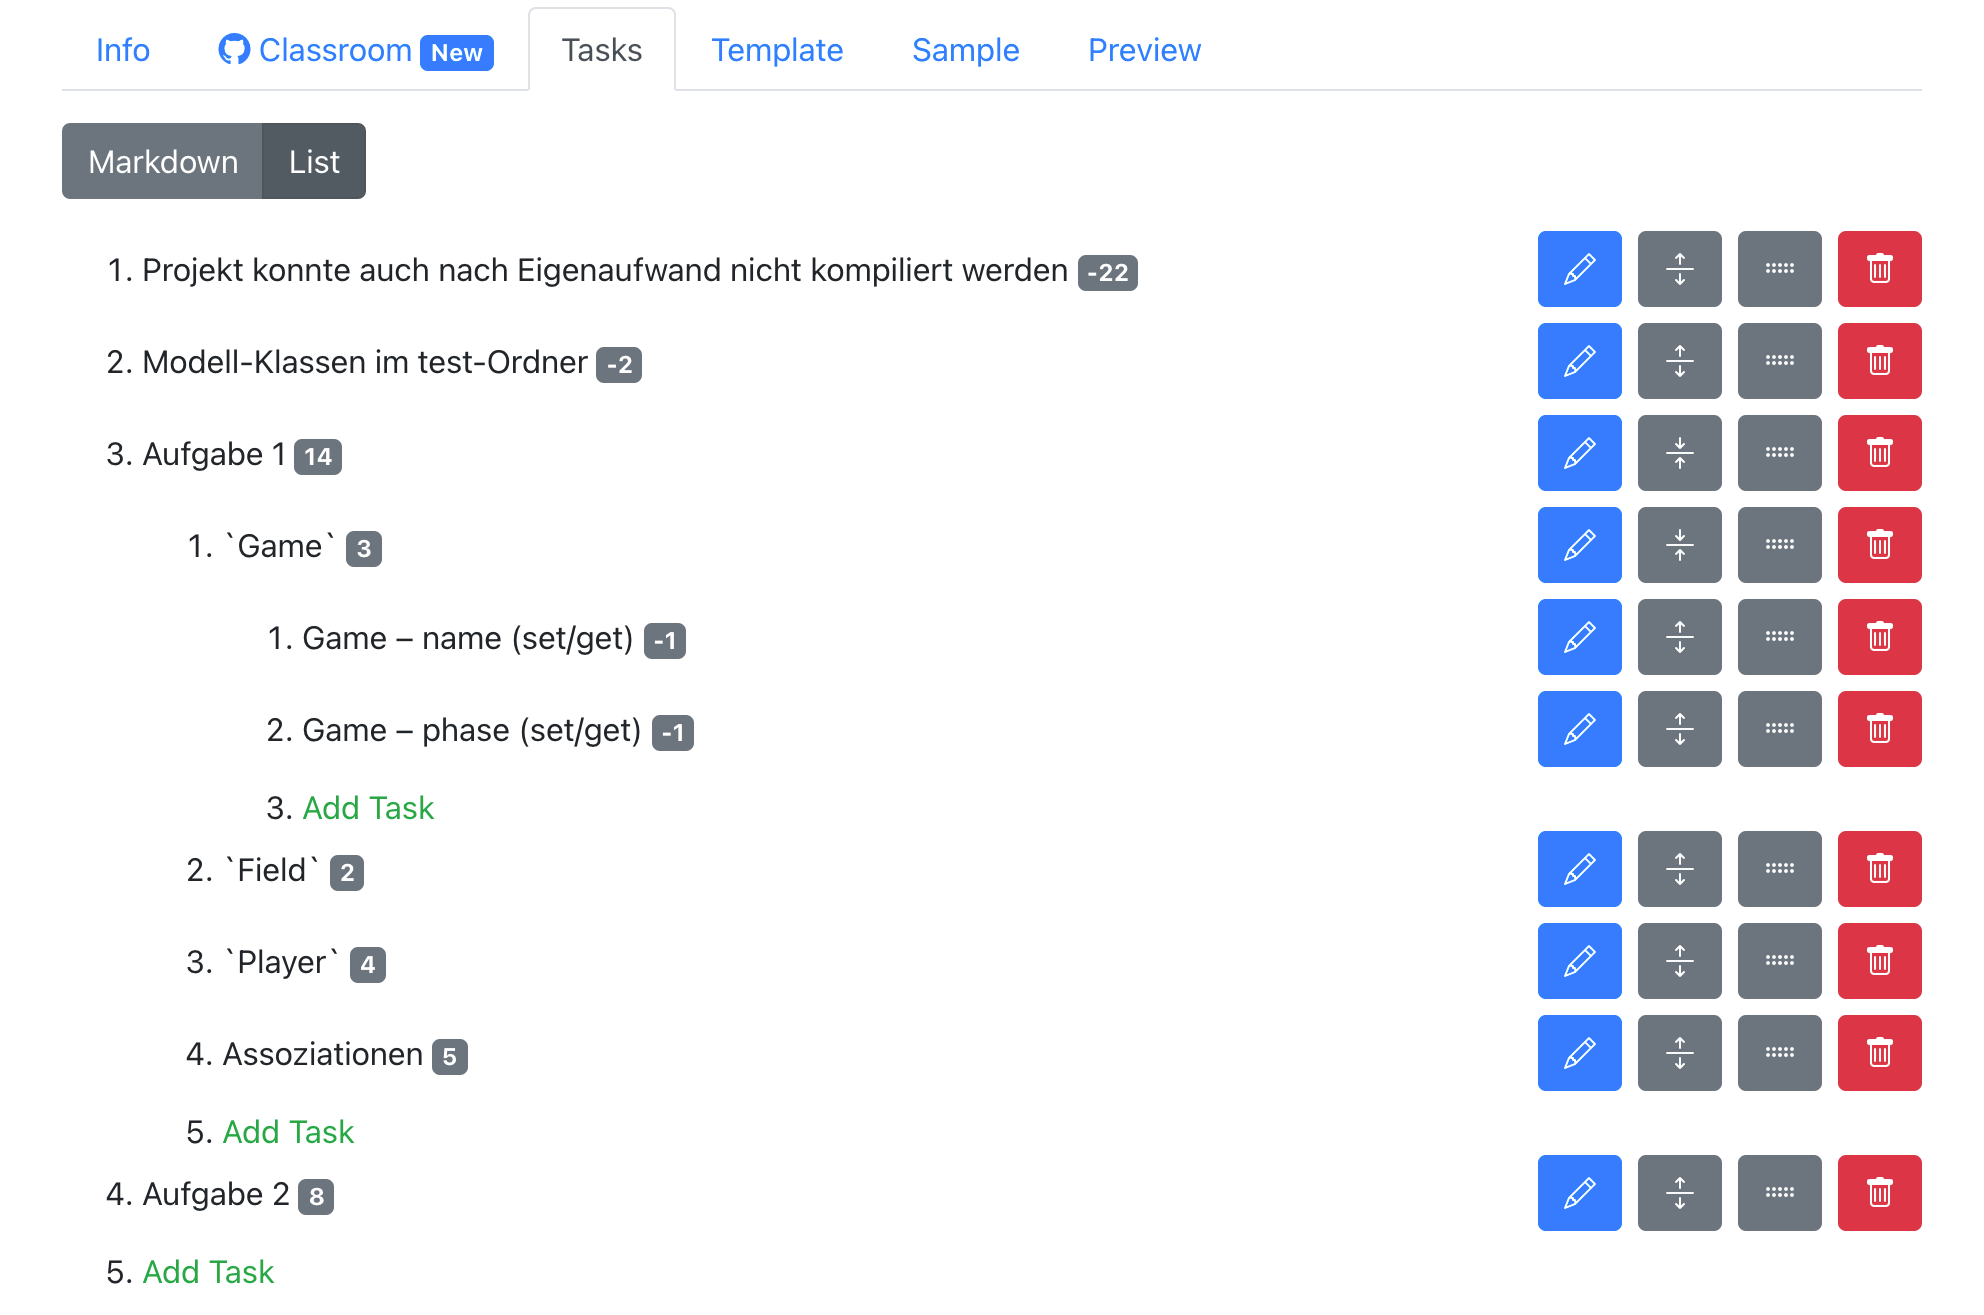
\includegraphics[width=\textwidth]{images/assignment-create-tasks-list}
    \caption{Baum-Editor für Teilaufgaben}
    \label{fig:assignment-create-tasks-list}
\end{figure}

Nun muss die Struktur des Aufgabenblatts anhand von Teilaufgaben, genannt Tasks, definiert werden.
Diese können beliebig geschachtelt und angeordnet werden, weshalb ein spezieller Editor für die Bearbeitung notwendig ist.
Abbildung~\ref{fig:assignment-create-tasks-list} zeigt, wie dieser in der Oberfläche aussieht.
Jeder Task besteht mindestens aus einer kurzen Beschreibung, die auch als Titel dienen kann, und einer Punktzahl.
In der Abbildung ist bereits erkennbar, dass eine Punktzahl nicht zwangsweise positiv sein muss.
Ein Task mit negativer Punktzahl wird als Abzug bezeichnet und kann besonders dann eingesetzt werden, wenn eine Aufgabe aus vielen ungeordneten Teilen besteht.
Dann ist es möglich, in einem Feedback nur die zutreffenden Abzüge darzustellen und damit die Übersichtlichkeit und Nachvollziehbarkeit zu verbessern.

Neben jedem Task werden vier Buttons angezeigt.
Der blaue Stift öffnet die Detailansicht des Tasks, die in den Abbildungen~\ref{fig:assignment-create-tasks-detail} dargestellt ist und im Folgenden beschrieben wird.
Mit dem Pfeile-Button kann ein Task aus- oder eingeklappt werden, um die Untertasks anzuzeigen oder zu verbergen.
Die nächste Schaltfläche kann verwendet werden, um die Reihenfolge der Tasks anzupassen oder Tasks unter andere zu verschieben.
Zuletzt erlaubt der Mülleimer-Button das Löschen eines Tasks.
Dabei handelt es sich nicht um eine sofortige Löschung, der Task wird lediglich als gelöscht markiert und kann wiederhergestellt werden, um eventuellen Datenverlust zu vermeiden.

\begin{figure}
    \centering
    \begin{subfigure}[t]{0.475\textwidth}
        \centering
        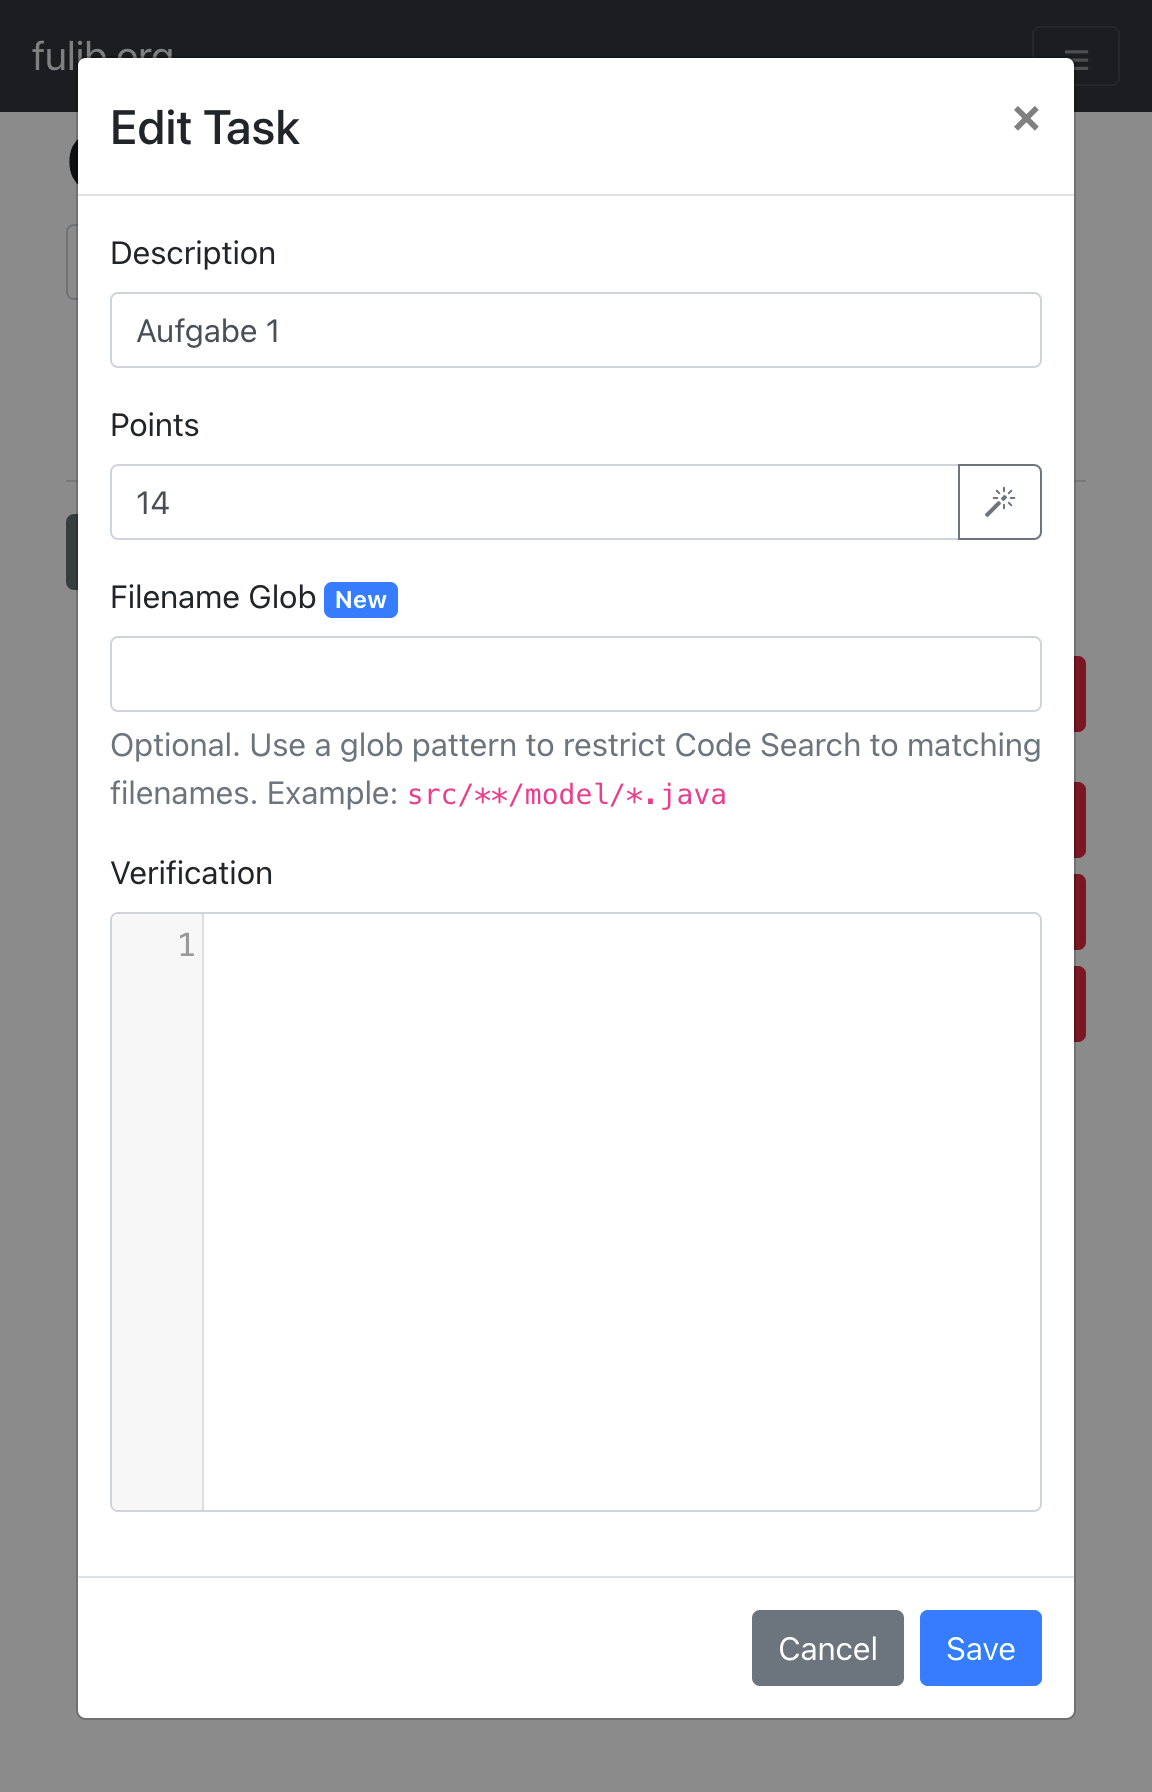
\includegraphics[width=\textwidth]{images/assignment-create-tasks-detail-1}
        \caption{Detailansicht eines positiven Tasks mit Untertasks}
        \label{fig:assignment-create-tasks-detail-1}
    \end{subfigure}
    \hfill
    \begin{subfigure}[t]{0.475\textwidth}
        \centering
        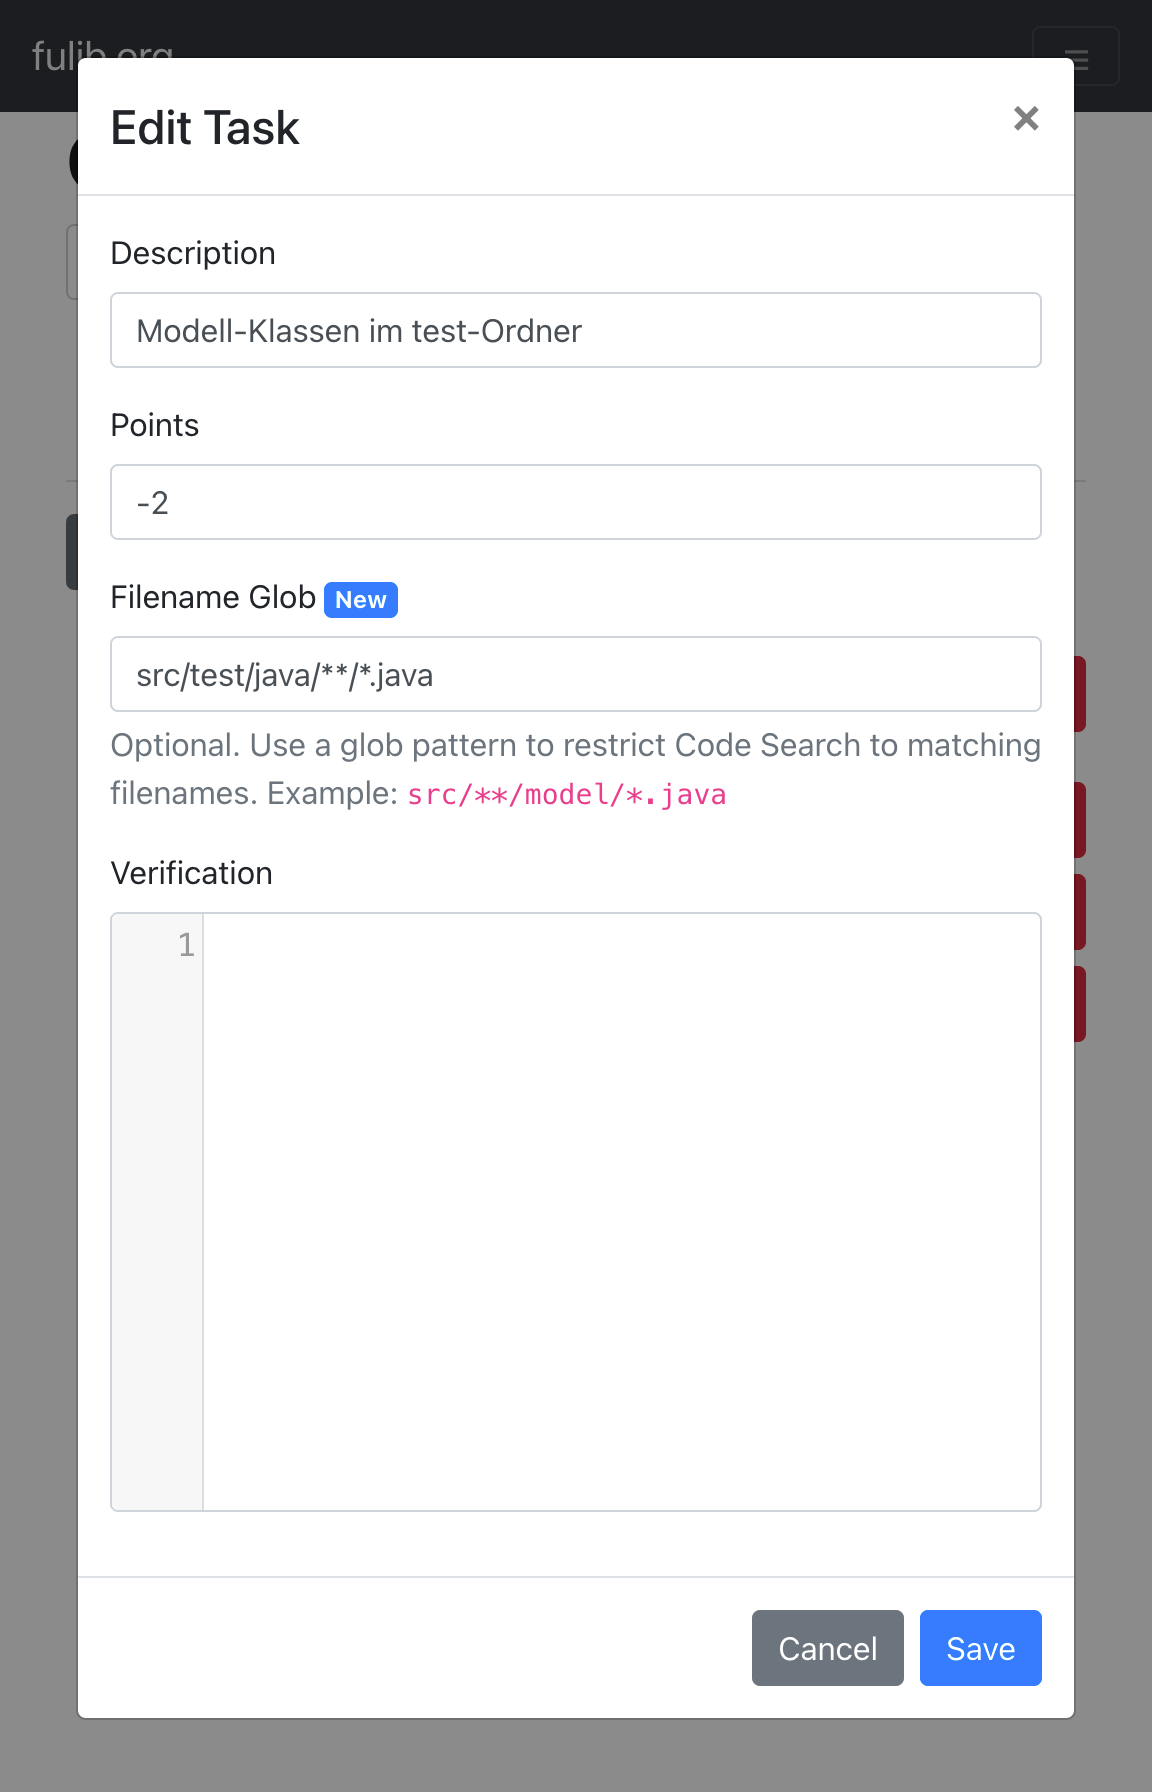
\includegraphics[width=\textwidth]{images/assignment-create-tasks-detail-2}
        \caption{Detailansicht eines negativen Tasks}
        \label{fig:assignment-create-tasks-detail-2}
    \end{subfigure}
    \caption{Detailansicht zweier Tasks}
    \label{fig:assignment-create-tasks-detail}
\end{figure}

Die Detailansichten eines positiven Tasks mit Untertasks und eines negativen Tasks sind jeweils in den Abbildungen~\ref{fig:assignment-create-tasks-detail-1} und~\ref{fig:assignment-create-tasks-detail-2} sichtbar.
In dem modalen Formular kann die Beschreibung und die Punktzahl eingestellt werden.
In der ersten Abbildung ist zu sehen, dass die Existenz von Unteraufgaben die automatische Berechnung der Punktzahl ermöglicht, weshalb der Zauberstab-Button neben dem Eingabefeld sichtbar ist.
Die Berechnung behandelt Unteraufgaben mit negativen Punktzahlen gesondert, indem jeweils deren absoluter Betrag verwendet wird.
Das optionale Eingabefeld \textbf{Filename Glob} ist für die in Abschnitt~\ref{subsec:code-search} beschriebene Code Search relevant und wird dort separat beschrieben.
Abbildung~\ref{fig:assignment-create-tasks-detail-2} zeigt eine Beispieleingabe.
Der Editor \textbf{Verification} wird für die automatische Bewertung mit fulibScenarios und dessen Pattern Matching-Erweiterung aus~\cite{bachelor-thesis} verwendet und ist in dieser Arbeit nicht weiter relevant.

\begin{figure}
    \centering
    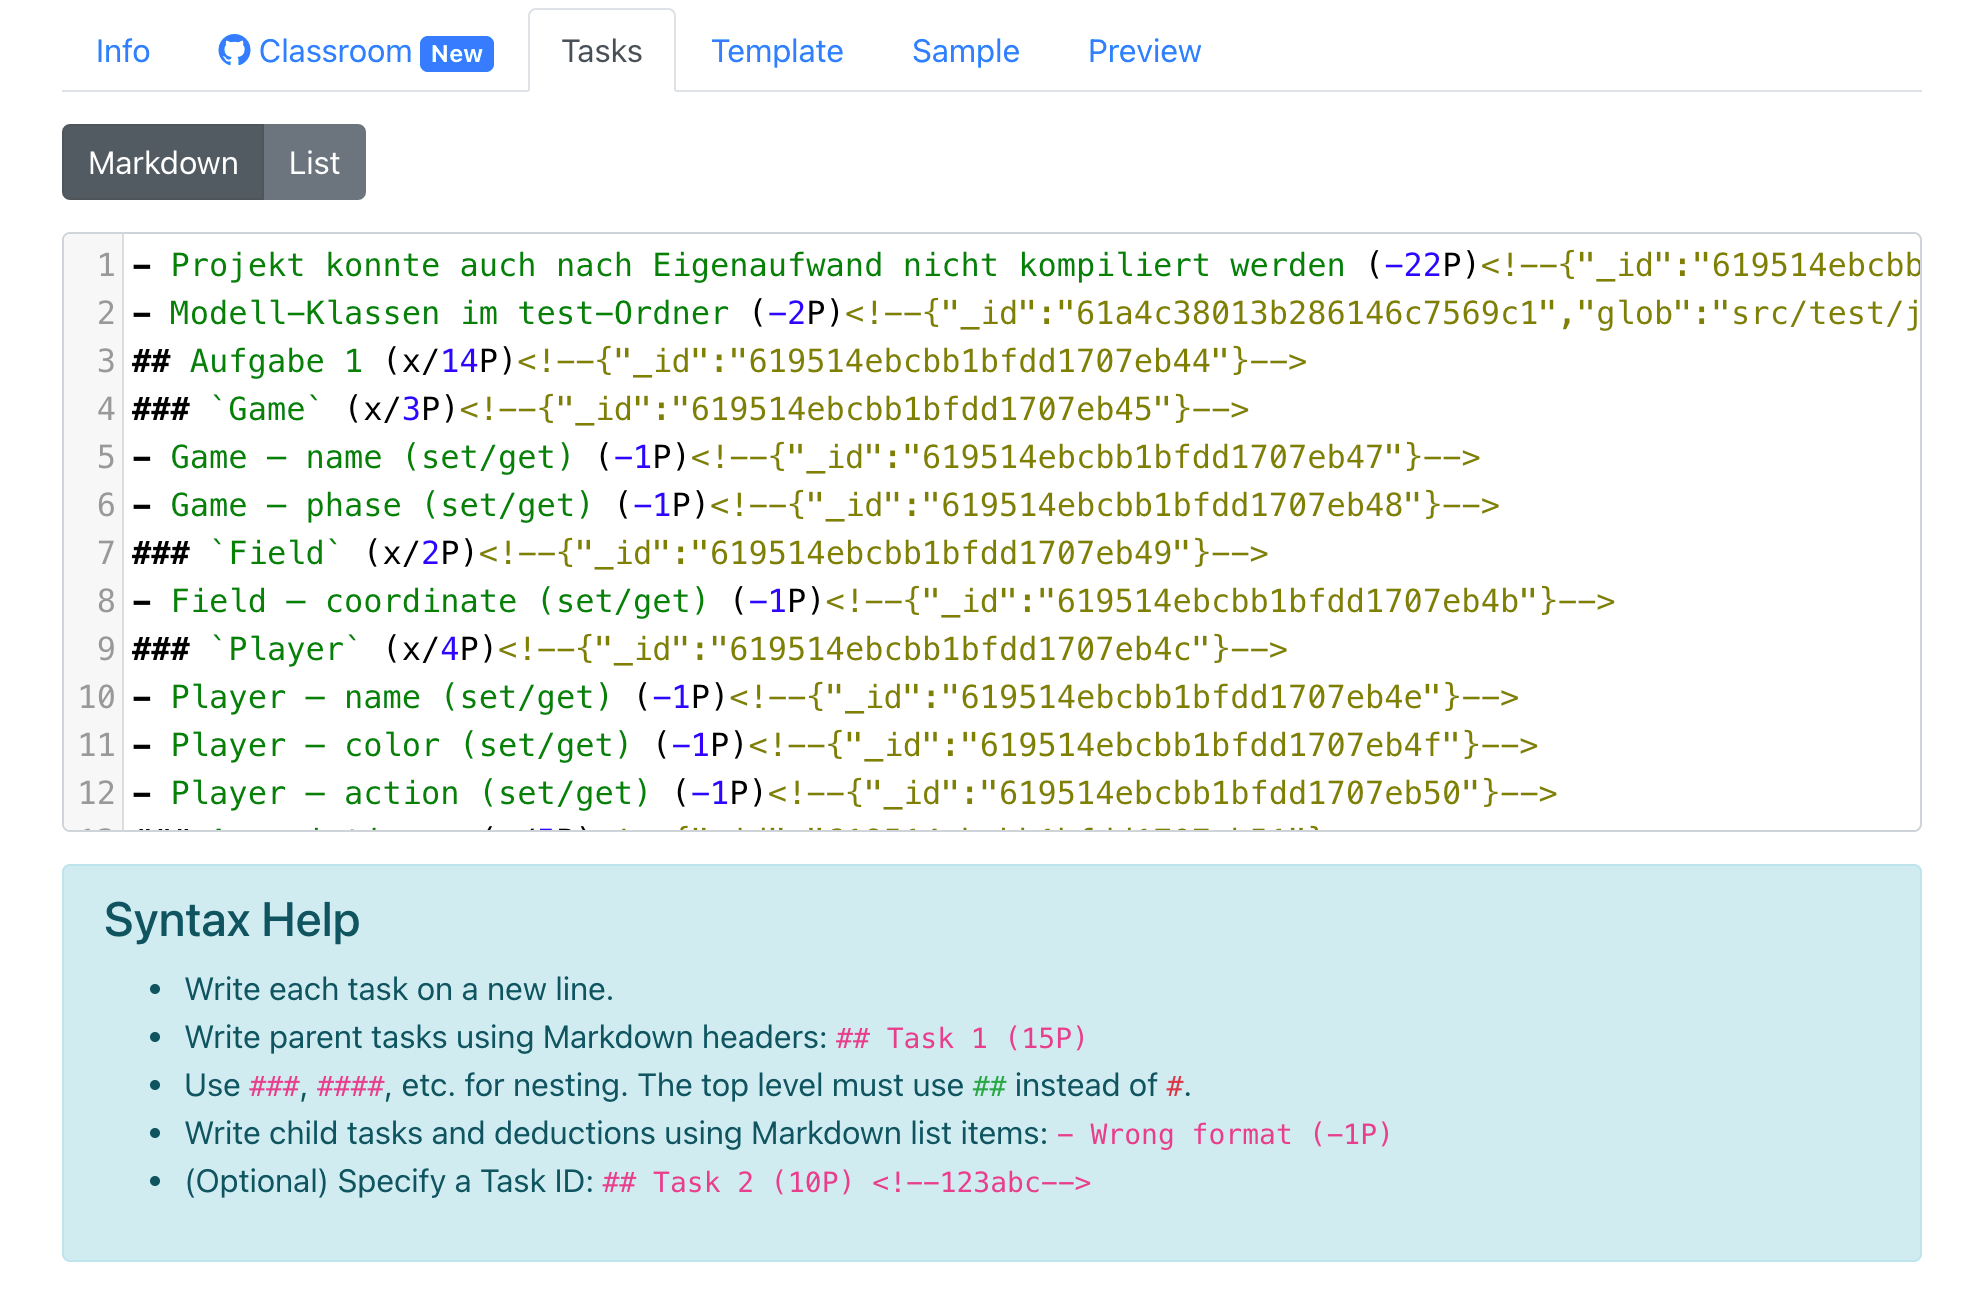
\includegraphics[width=\textwidth]{images/assignment-create-tasks-markdown}
    \caption{Markdown-Editor für Teilaufgaben}
    \label{fig:assignment-create-tasks-markdown}
\end{figure}

Die Schaltfläche zum Wechseln zwischen \textbf{Markdown} und \textbf{List} erlaubt die Bearbeitung der Tasks in einer auf Markdown basierenden Textformat.
Abbildung~\ref{fig:assignment-create-tasks-markdown} zeigt einen Ausschnitt der Teilaufgabenliste aus Abbildung~\ref{fig:assignment-create-tasks-list} in diesem Format sowie der zugehörige Hilfetext zur Erklärung.
Das Format kann in wenigen Sätzen beschrieben werden.
Jeder Task wird in eine neue Zeile geschrieben, die entweder der Listensyntax (\code{-} am Anfang) oder der Überschriftensyntax (Zwei oder mehrere \code{\#} am Anfang) von Markdown folgt.
Nach dem einleitenden Zeichen folgt die Beschreibung und die Punktzahl, optional mit \code{x/} vorangestellt und/oder \code{P} nachgestellt, in Klammern.
Am Ende der Zeile kann ein \ac{html}-Kommentare weitere Daten des Tasks wie dessen \ac{id} und Dateinamen-Glob in \ac{json} kodiert enthalten.
Folgt eine Zeile nicht diesem Format, wird sie rot markiert, um den Benutzer auf das Problem hinzuweisen.

Das Format wurde gewählt, da die Bewertungsrichtlinien der Veranstaltung Programmieren und Modellieren bereits vor Beginn dieser Arbeit in ähnlichem Format vorlagen.
Diese Richtlinien haben ihre Ursprünge aus der Verwendung von GitHub, wo Issues, Pull Requests und Kommentare in Markdown verfasst werden können und dann in Listenform mit Teilüberschriften dargestellt werden.
Meist war es während der Evaluation möglich, die Bewertungsrichtlinien einzusetzen und mit wenigen Änderungen dem Format anzupassen.

Die Registerkarten \textbf{Template} und \textbf{Sample} aus Abbildung~\ref{fig:assignment-create-head} werden an dieser Stelle nicht näher erläutert.
Es handelt sich um spezifische Einstellungen für die Bewertung von Szenarien aus~\cite{bachelor-thesis}, die für die Zwecke dieser Arbeit nicht anwendbar sind.

\begin{figure}
    \centering
    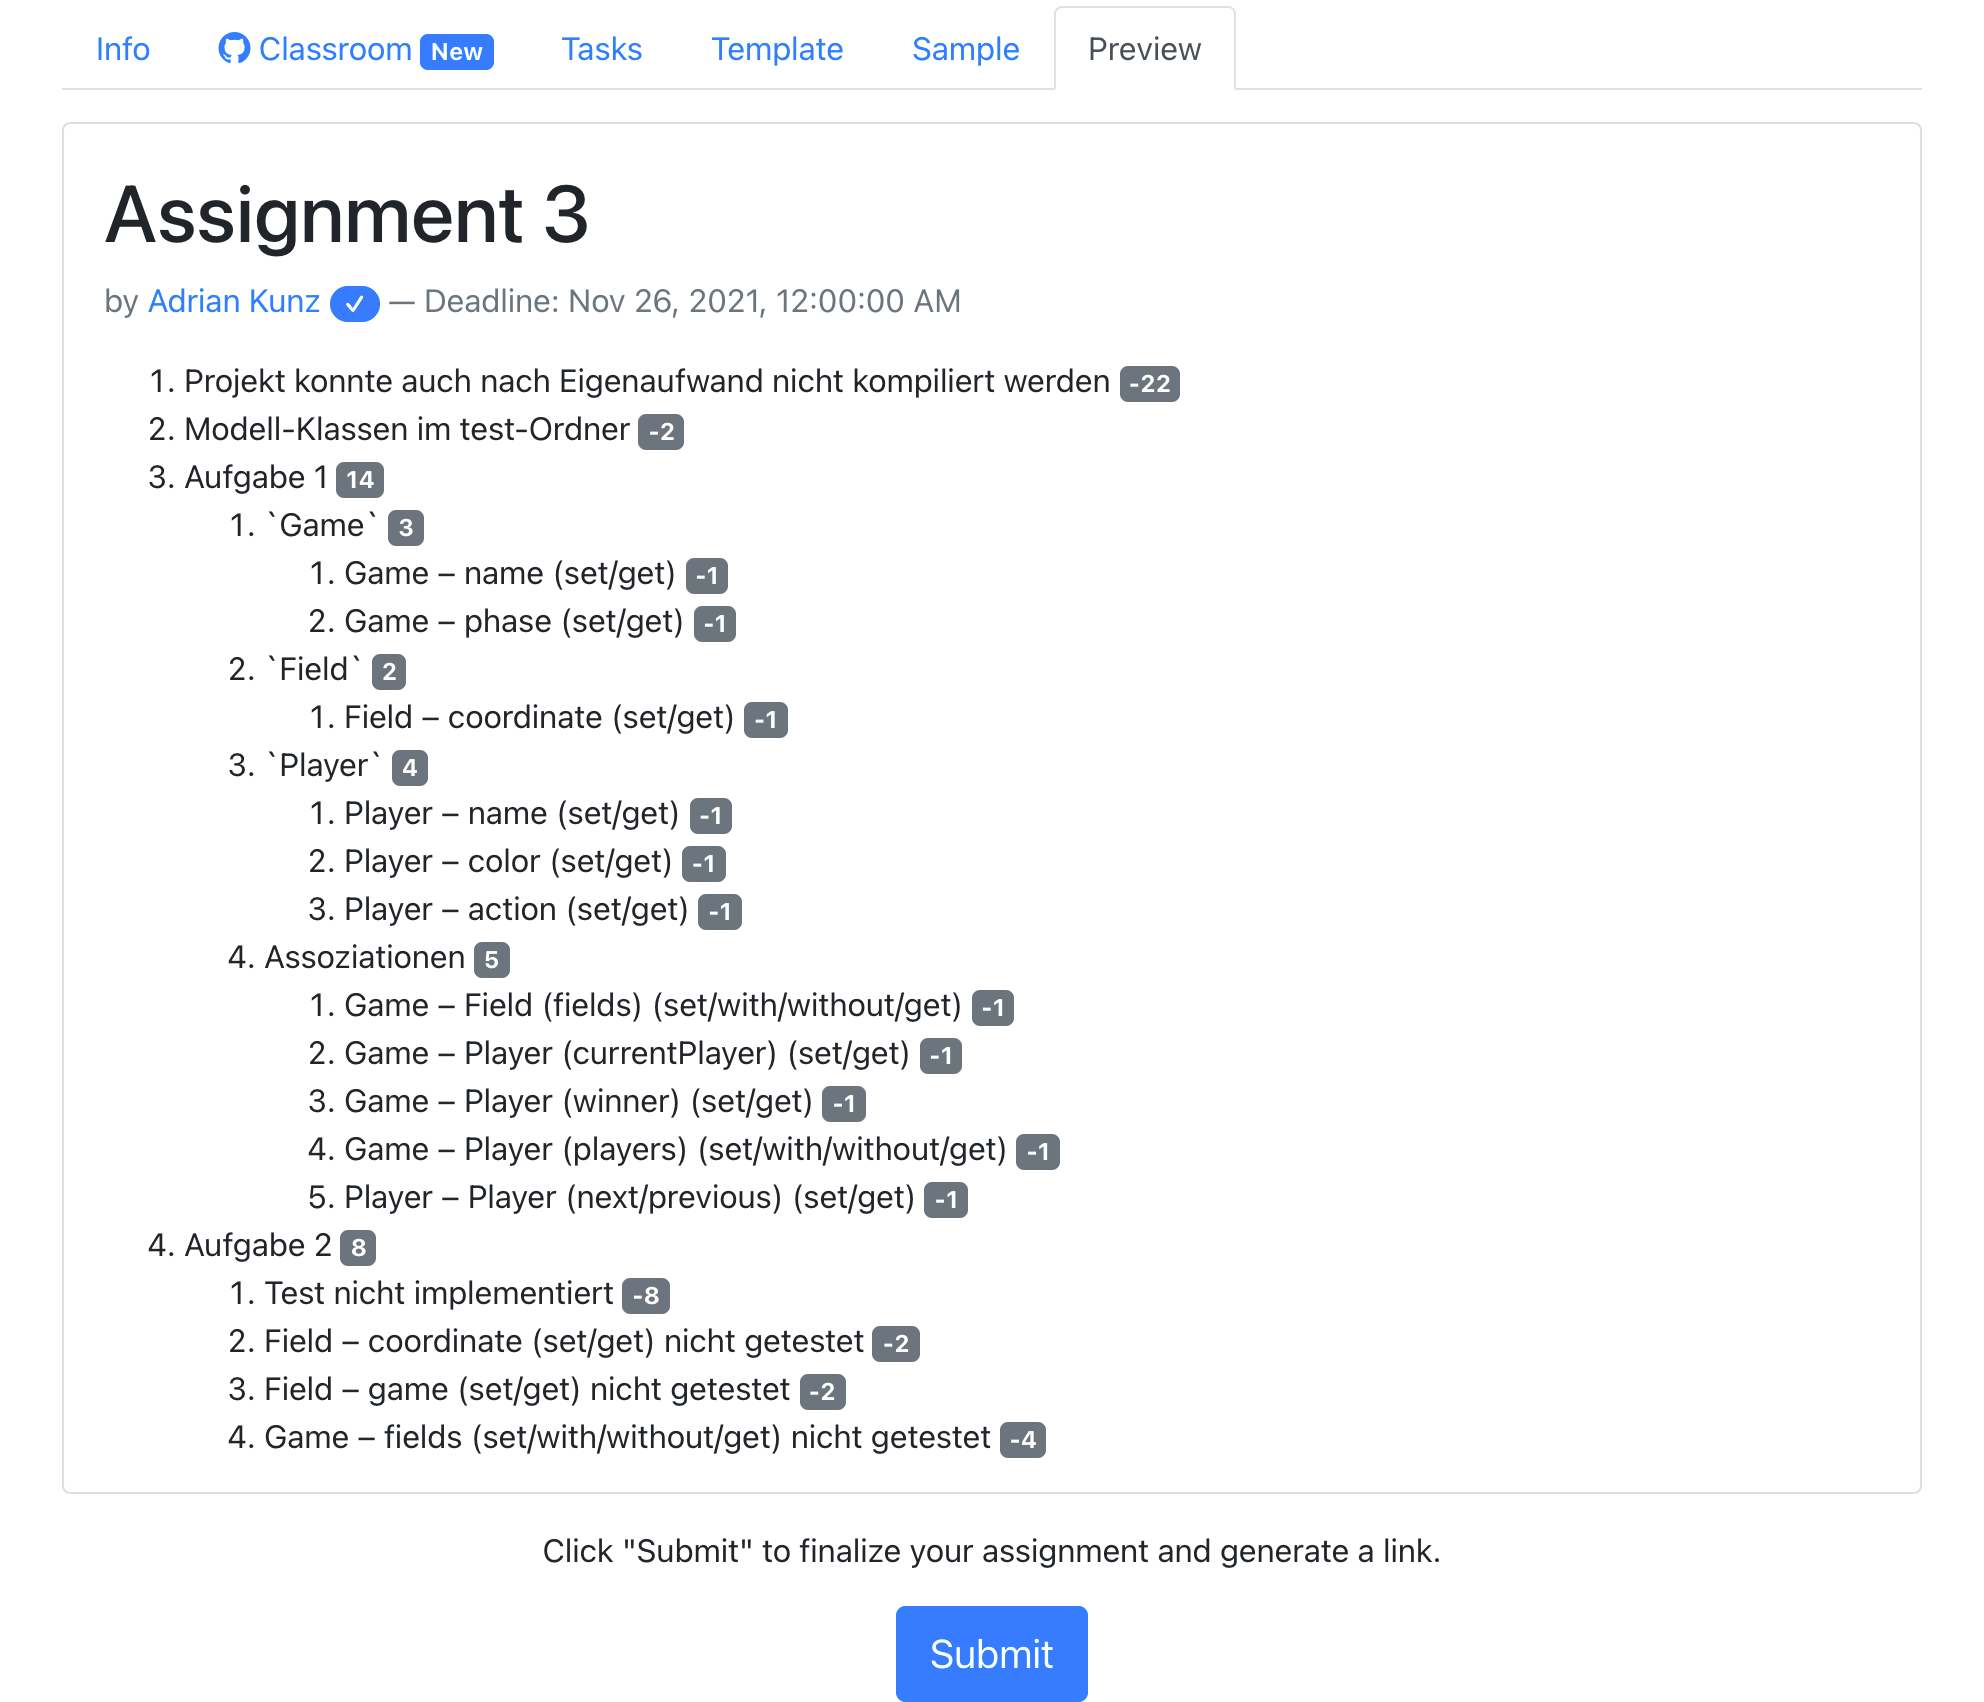
\includegraphics[width=\textwidth]{images/assignment-create-preview}
    \caption{Abschließende Vorschau vor Erstellen eines Assignments}
    \label{fig:assignment-create-preview}
\end{figure}

Der letzte Schritt der Assignment-Erstellung befindet sich auf der Registerkarte \textbf{Preview}, welche eine Übersicht über das Assignment anhand einer Vorschau anzeigt.
In Abbildung~\ref{fig:assignment-create-preview} wird diese dargestellt.
In der Vorschau werden Titel, Autor, Abgabefrist und, falls vorhanden, die Beschreibung angezeigt.
Sämtliche Teilaufgaben werden in einer geschachtelten Liste mit Beschreibung und Punktzahl präsentiert.
Schließlich kann das Assignment mit dem \textbf{Submit}-Button erstellt und veröffentlicht werden.

\begin{figure}
    \centering
    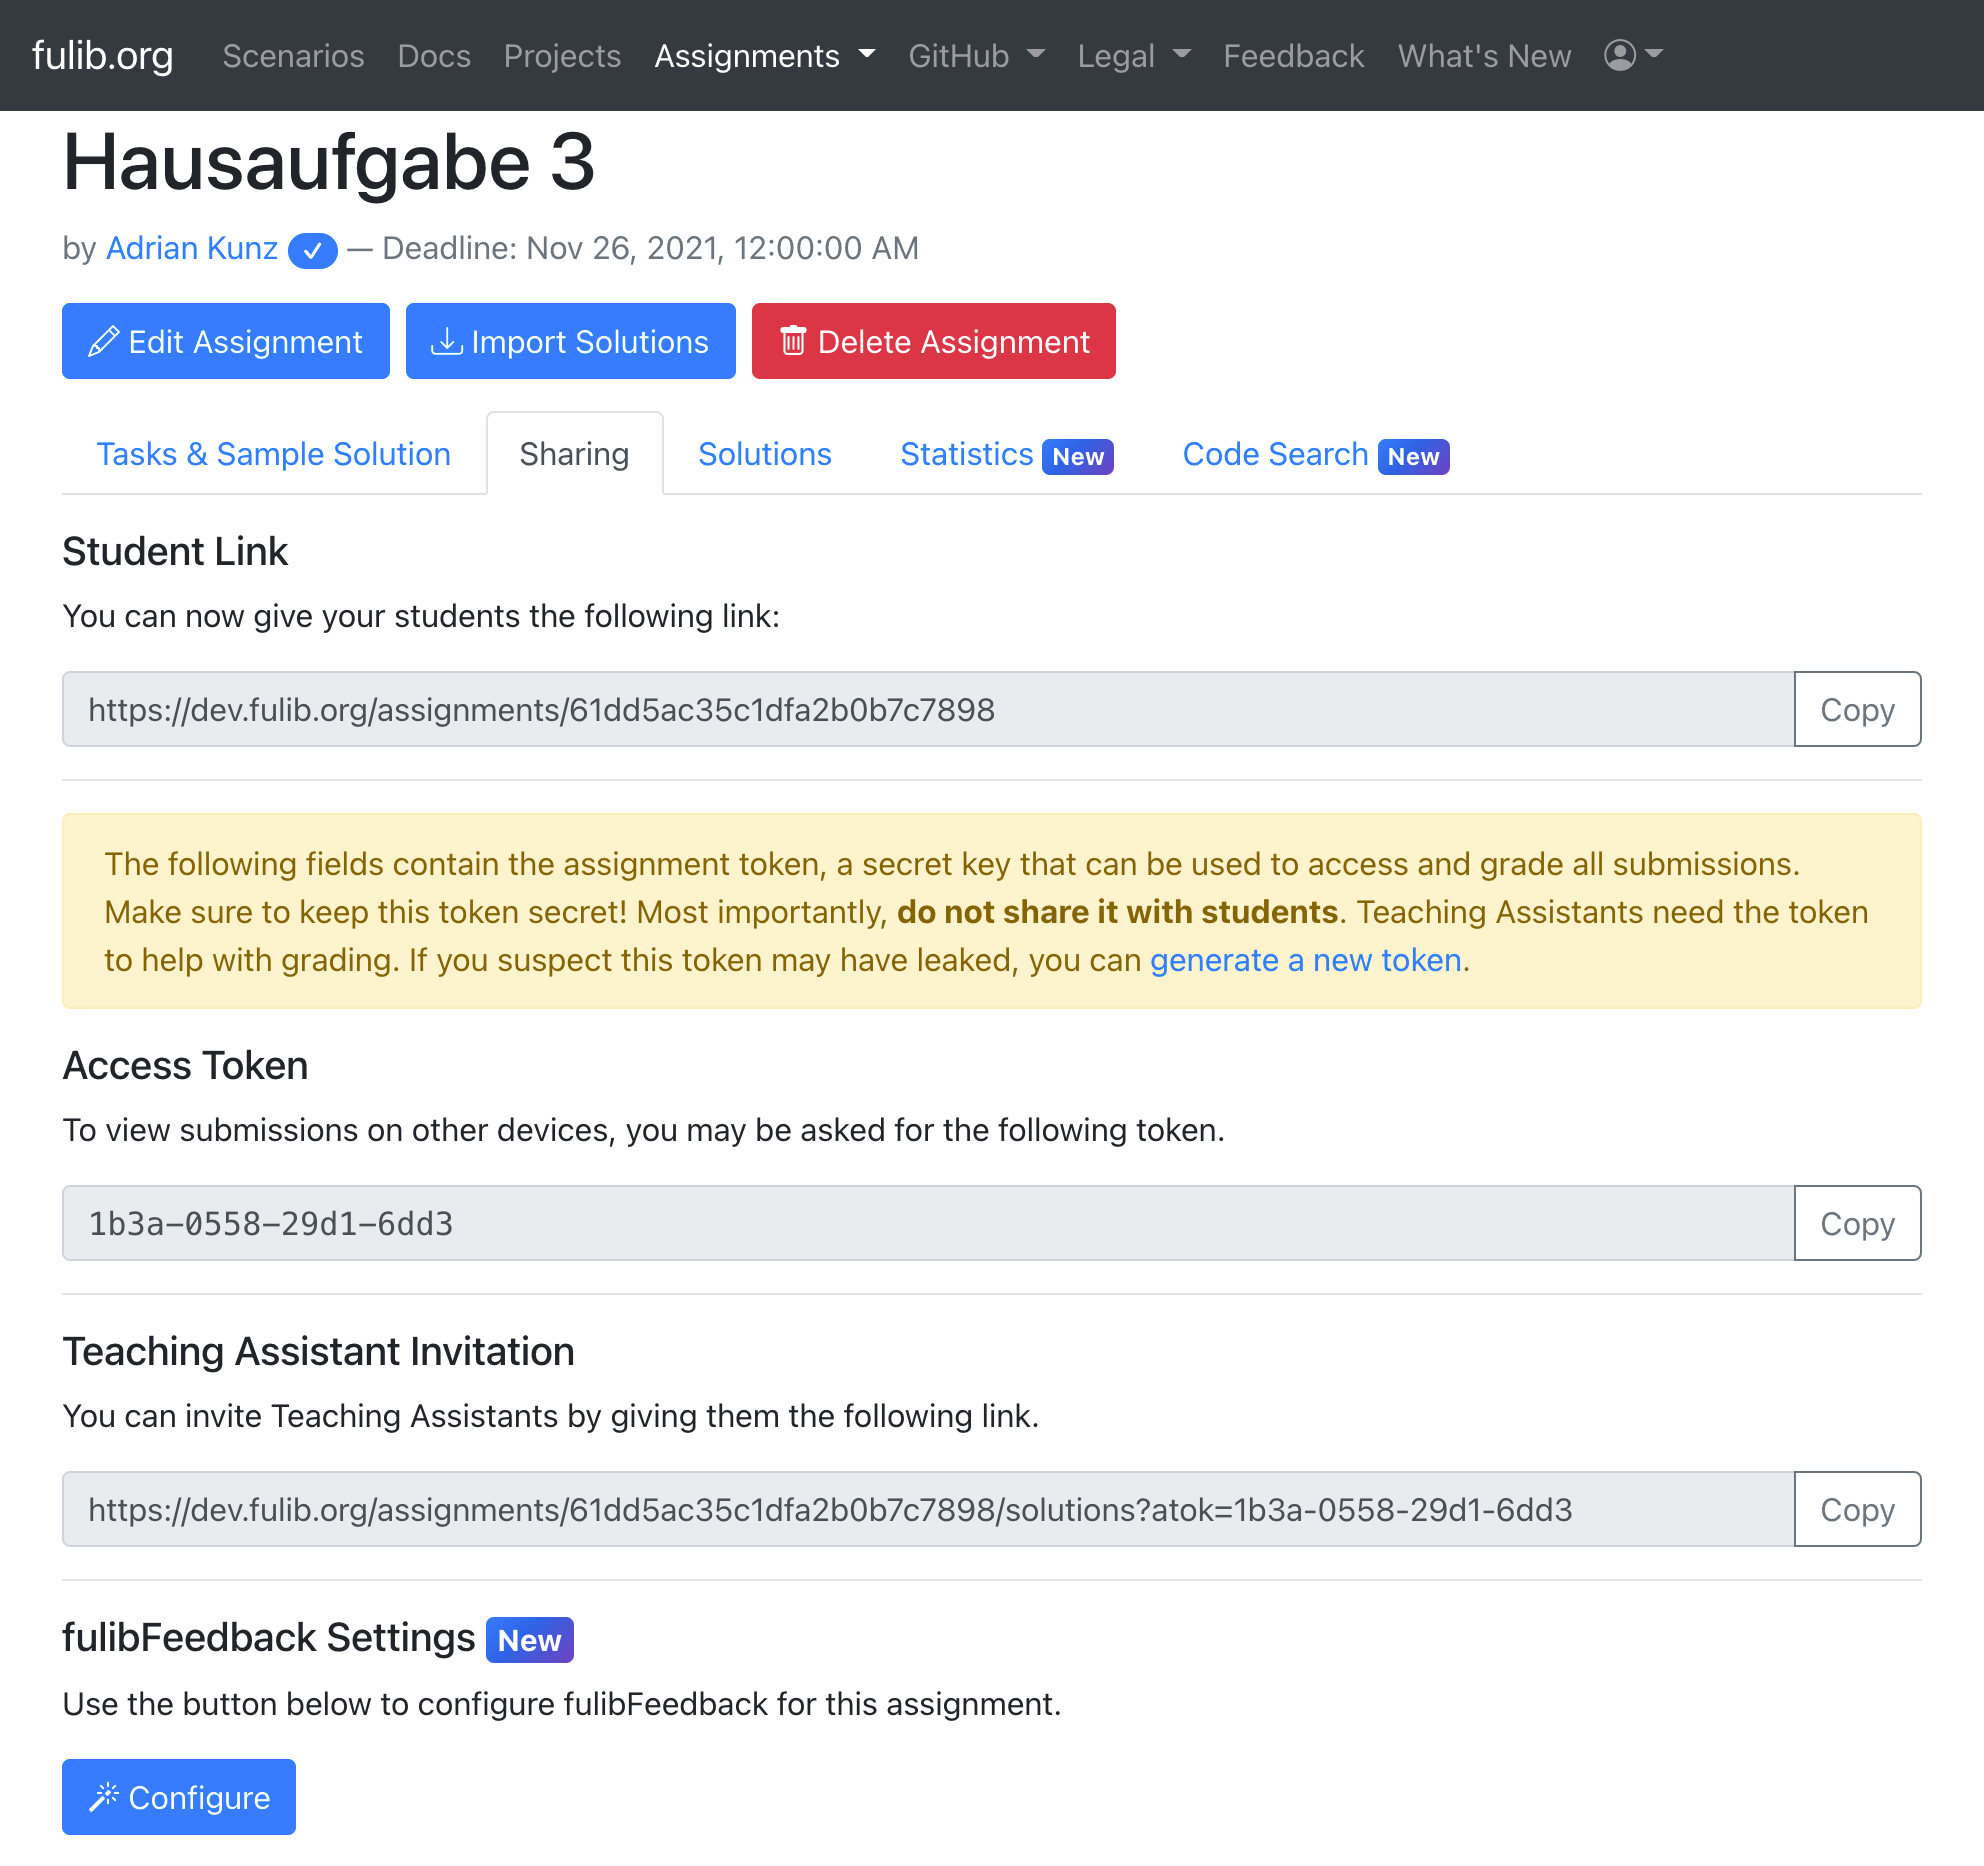
\includegraphics[width=\textwidth]{images/assignment-share}
    \caption{Teilen eines Assignments}
    \label{fig:assignment-share}
\end{figure}

Die Veröffentlichung findet über den \textbf{Sharing}-Tab statt, der sich direkt nach Erstellen des Assignments öffnet und in Abbildung~\ref{fig:assignment-share} dargestellt ist.
Der \textbf{Student Link} wurde hauptsächlich in~\cite{bachelor-thesis} eingesetzt, da dieser zur Vergabe an die Studierenden vorgesehen war.
In dieser Arbeit interagieren diese jedoch nicht mit der Oberfläche, weshalb der Link nicht benötigt wird.
Das \textbf{Access Token} dient der Zugriffskontrolle, da mit diesem sämtliche Aktionen von Bewertenden durchgeführt werden.
Daher muss sichergestellt werden, dass es nicht an Studierende gelangt, wie die Warnmeldung beschreibt.
Bewertende benötigen folglich das Token und können es über den teilbaren \textbf{Teaching Assistant Invitation}-Link erhalten.
Der Button \textbf{Configure} wird für fulibFeedback eingesetzt und wird in Abschnitt~\ref{sec:fulibFeedback} erneut erwähnt.

\subsection{Bewertung}\label{subsec:grading}

Sobald die Bewertenden den Einladungslink für ein Assignment erhalten haben, können sie mit der Bewertung beginnen.
Nachfolgend werden einige Schritte beschrieben, die dafür notwendig sind.
Es handelt sich um wiederholende Abläufe, die jedoch nach kurzer Eingwöhnungszeit eine effiziente Arbeitsweise erlauben.
Dies wird in Kapitel~\ref{ch:evaluation} näher beleuchtet.

\subsubsection{Abgabentabelle}

Begonnen wird in der Tabelle mit allen Abgaben unter dem Tab \textbf{Solutions}.
Diese ist in Abbildung~\ref{fig:assignment-solutions-table} ausgeschnitten dargestellt.

\begin{figure}
    \centering
    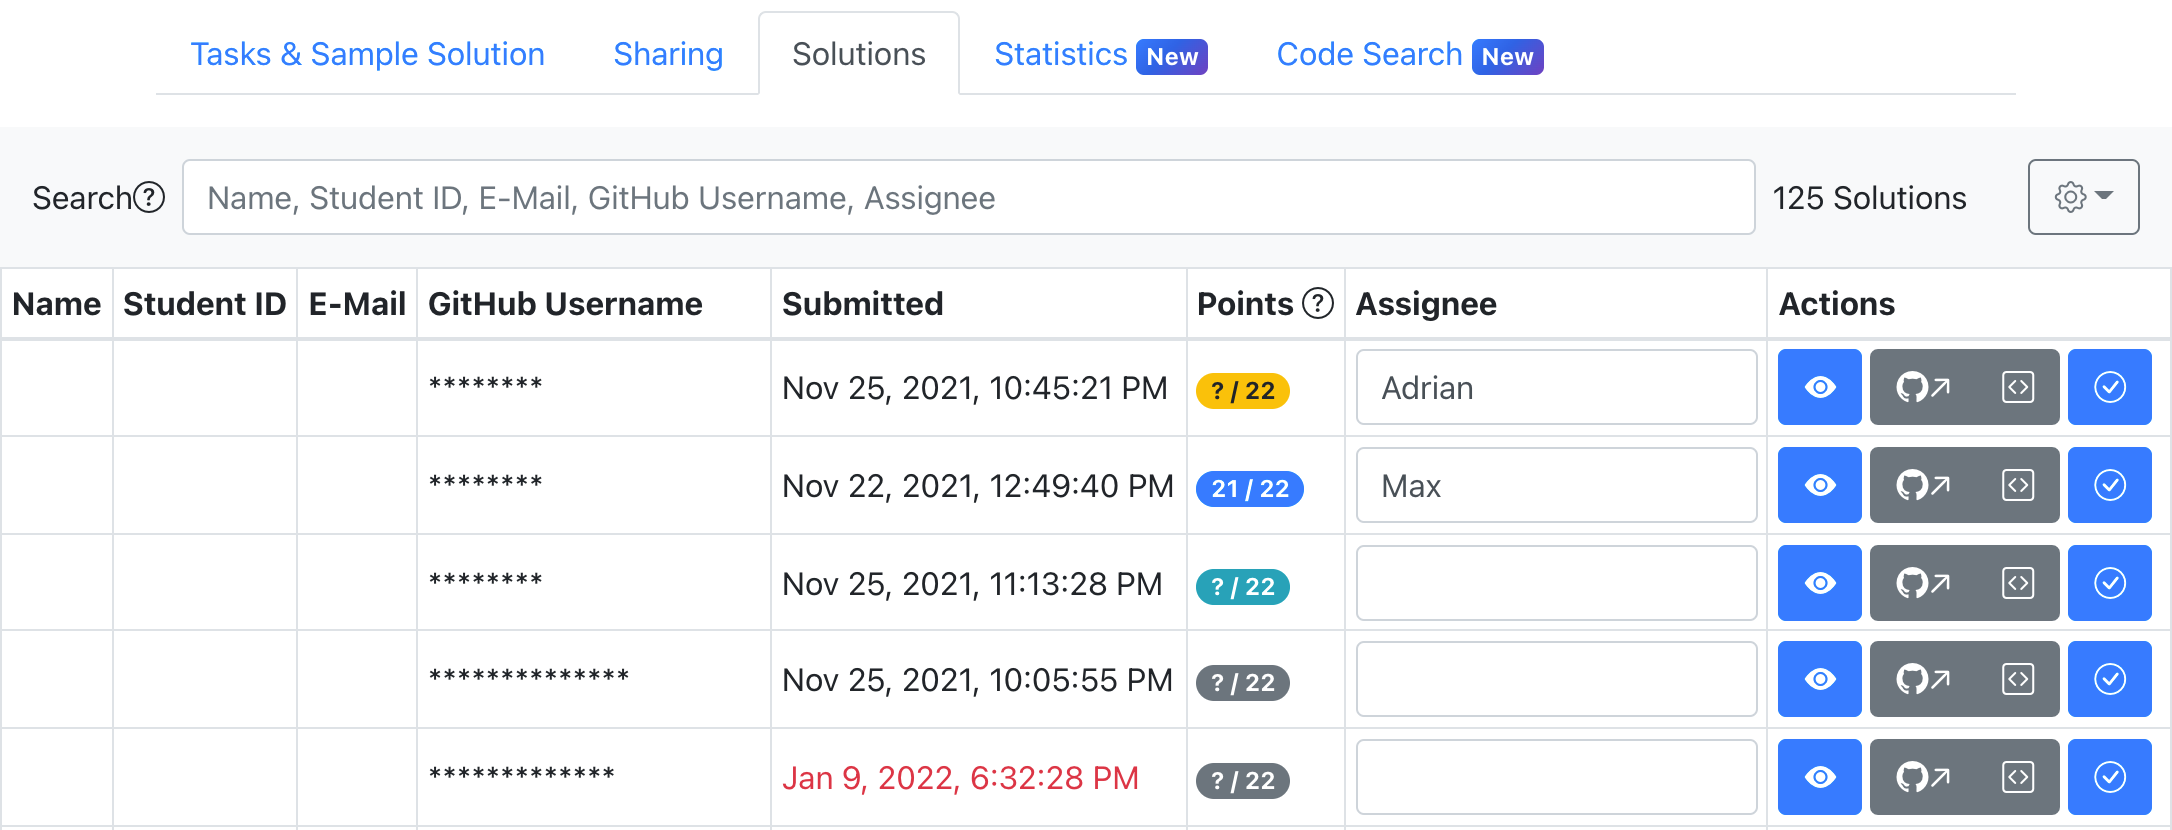
\includegraphics[width=\textwidth]{images/assignment-solutions-table}
    \caption{Tabelle mit allen Abgaben nach dem Import}
    \label{fig:assignment-solutions-table}
\end{figure}

In diesem Fall wurden die Lösungen automatisch nach Ablauf der Abgabefrist aus GitHub Classroom importiert.
Die Tabelle gibt Auskunft über den GitHub-Benutzernamen\footnote{
    Für diese Abbildung wurden die Benutzernamen durch \texttt{*}-Symbole ersetzt.
} und das Abgabedatum (\textbf{Submitted}), welches dem letzten Push\footnote{
    Bezeichnet die Aktion der Versionskontroll-Software Git, bei der lokale Commits auf den Remote-Server hochgeladen werden.
}-Zeitpunkt vor der Frist entspricht.
Bei einem nachträglichen manuellem Import ist es möglich, dass die Push-Zeit nach der Abgabefrist liegt.
In diesem Fall wird das Abgabedatum rot markiert.
Name, Matrikelnummer (\textbf{Student \acs{id}}) und E-Mail-Adresse können nicht von GitHub Classroom ermittelt werden, weshalb sie in der Tabelle leer sind.

Die Punktzahl ist zunächst mit \texttt{?} als unausgewertet markiert.
In der Abbildung wurden bereits einige Bewertungen vorgenommen, weshalb die zweite Person eine abschließende Punktzahl von 21 erhalten hat.
Die gelb hinterlegte Punktzahl deutet an, dass eine Bewertung dieser Abgabe begonnen wurde, aber noch kein Feedback versendet wurde und daher keine Punktzahl feststeht.
Eine türkise Farbe markiert Abgaben, die zwar noch nicht händisch bewertet wurden, aber in denen eine automatisch angelegte Bewertung von Code Search vorhanden ist.
In Abgaben mit grauer Punktzahl ist keinerlei Bewertung vorhanden.
Das Fragezeichen-Symbol neben \textbf{Points} gibt Auskunft über diese Farbgebung.

Über die Textfelder unter \textbf{Assignee} können sich die Bewertenden die Abgaben zuordnen, für die sie zuständig sind.
Dadurch wird sichergestellt, dass nicht versehentlich eine Abgabe von mehreren Bewertenden betrachtet wird.
Die Textfelder bieten eine einfache Form der Autovervollständigung, sodass bei Eingabe weniger Buchstaben bereits der volle Name eines Bewertenden vorgeschlagen wird, sofern dieser bereits an einer anderen Stelle eingetragen war.

Mit der Suchleiste kann die Tabelle nach verschiedenen Kriterien gefiltert werden.
Beispielsweise können Bewertende durch Eingabe ihres Namens nur die ihnen zugewiesenen Abgaben anzeigen, um für Übersicht zu sorgen.
Die Syntax der Suche ist komplexer als eine einfache Textsuche, weshalb das Fragezeichen-Symbol eine detaillierte Beschreibung der Syntax anzeigen kann.

Unter den \textbf{Actions} befinden sich die wichtigsten Aktionen, die für die Bewertung einer Abgabe relevant sind.
Mit dem Augen-Button kann die Detailansicht der Abgabe geöffnet werden, in der die Bewertung einzelner Teilaufgaben stattfindet.
Dies ist Inhalt des folgenden Abschnitts.
Der graue GitHub-Button öffnet das Repository, von dem die Lösung importiert wurde, auf GitHub und zeigt dabei den Stand des letzten Commits vor der Abgabefrist.
Der Button mit eingerahmten spitzen Klammern öffnet die Lösung sofort in einer \ac{ide}, indem das GitHub-Repository gecloned\footnote{
    Git-Bezeichnung für das Kopieren eines Online-Repositories in einen lokalen Ordner.
} wird.
Mit dem Einstellungs-Button neben der Suchleiste kann zwischen verschiedenen \acp{ide} (\ac{vsc}, Code-OSS und VSCodium\footnote{
    Jeweils alternative quelloffene Builds von \ac{vsc} ohne Microsoft-Branding.
}) und Clone-Protokollen (https und ssh) gewählt werden.
Der blaue Button mit eingekreistem Haken wird in einem späteren Abschnitt für das Versenden des Feedbacks verwendet.

\subsubsection{Abgabe-Detailansicht}

\begin{figure}
    \centering
    
\includegraphics[width=\textwidth]{images/solution-head}
    \caption{Kopf der Abgabe-Detailansicht}
    \label{fig:solution-head}
\end{figure}


Die Detailansicht einer Abgabe öffnet sich nach Klicken des Augen-Buttons in der Abgabetabelle.
In Abbildung~\ref{fig:solution-head} ist sichtbar, dass auch diese Ansicht wieder in mehrere Tabs aufgeteilt ist, um übersichtlich zu bleiben.
In der Kopfzeile wird der Name\footnote{
    In Abbildung~\ref{fig:solution-head} wurde der GitHub-Benutzername erneut durch \texttt{*}-Symbole ersetzt.
} des Studierenden und die Abgabezeit stets angezeigt.
Für die Bewertung ist hauptsächlich der Tab \textbf{Solution \& Tasks} wichtig.
Die Teilaufgaben werden wieder in einer Baumansicht dargestellt, wie in Abbildung~\ref{fig:solution-tasks} erkennbar ist.

\begin{figure}
    \centering
    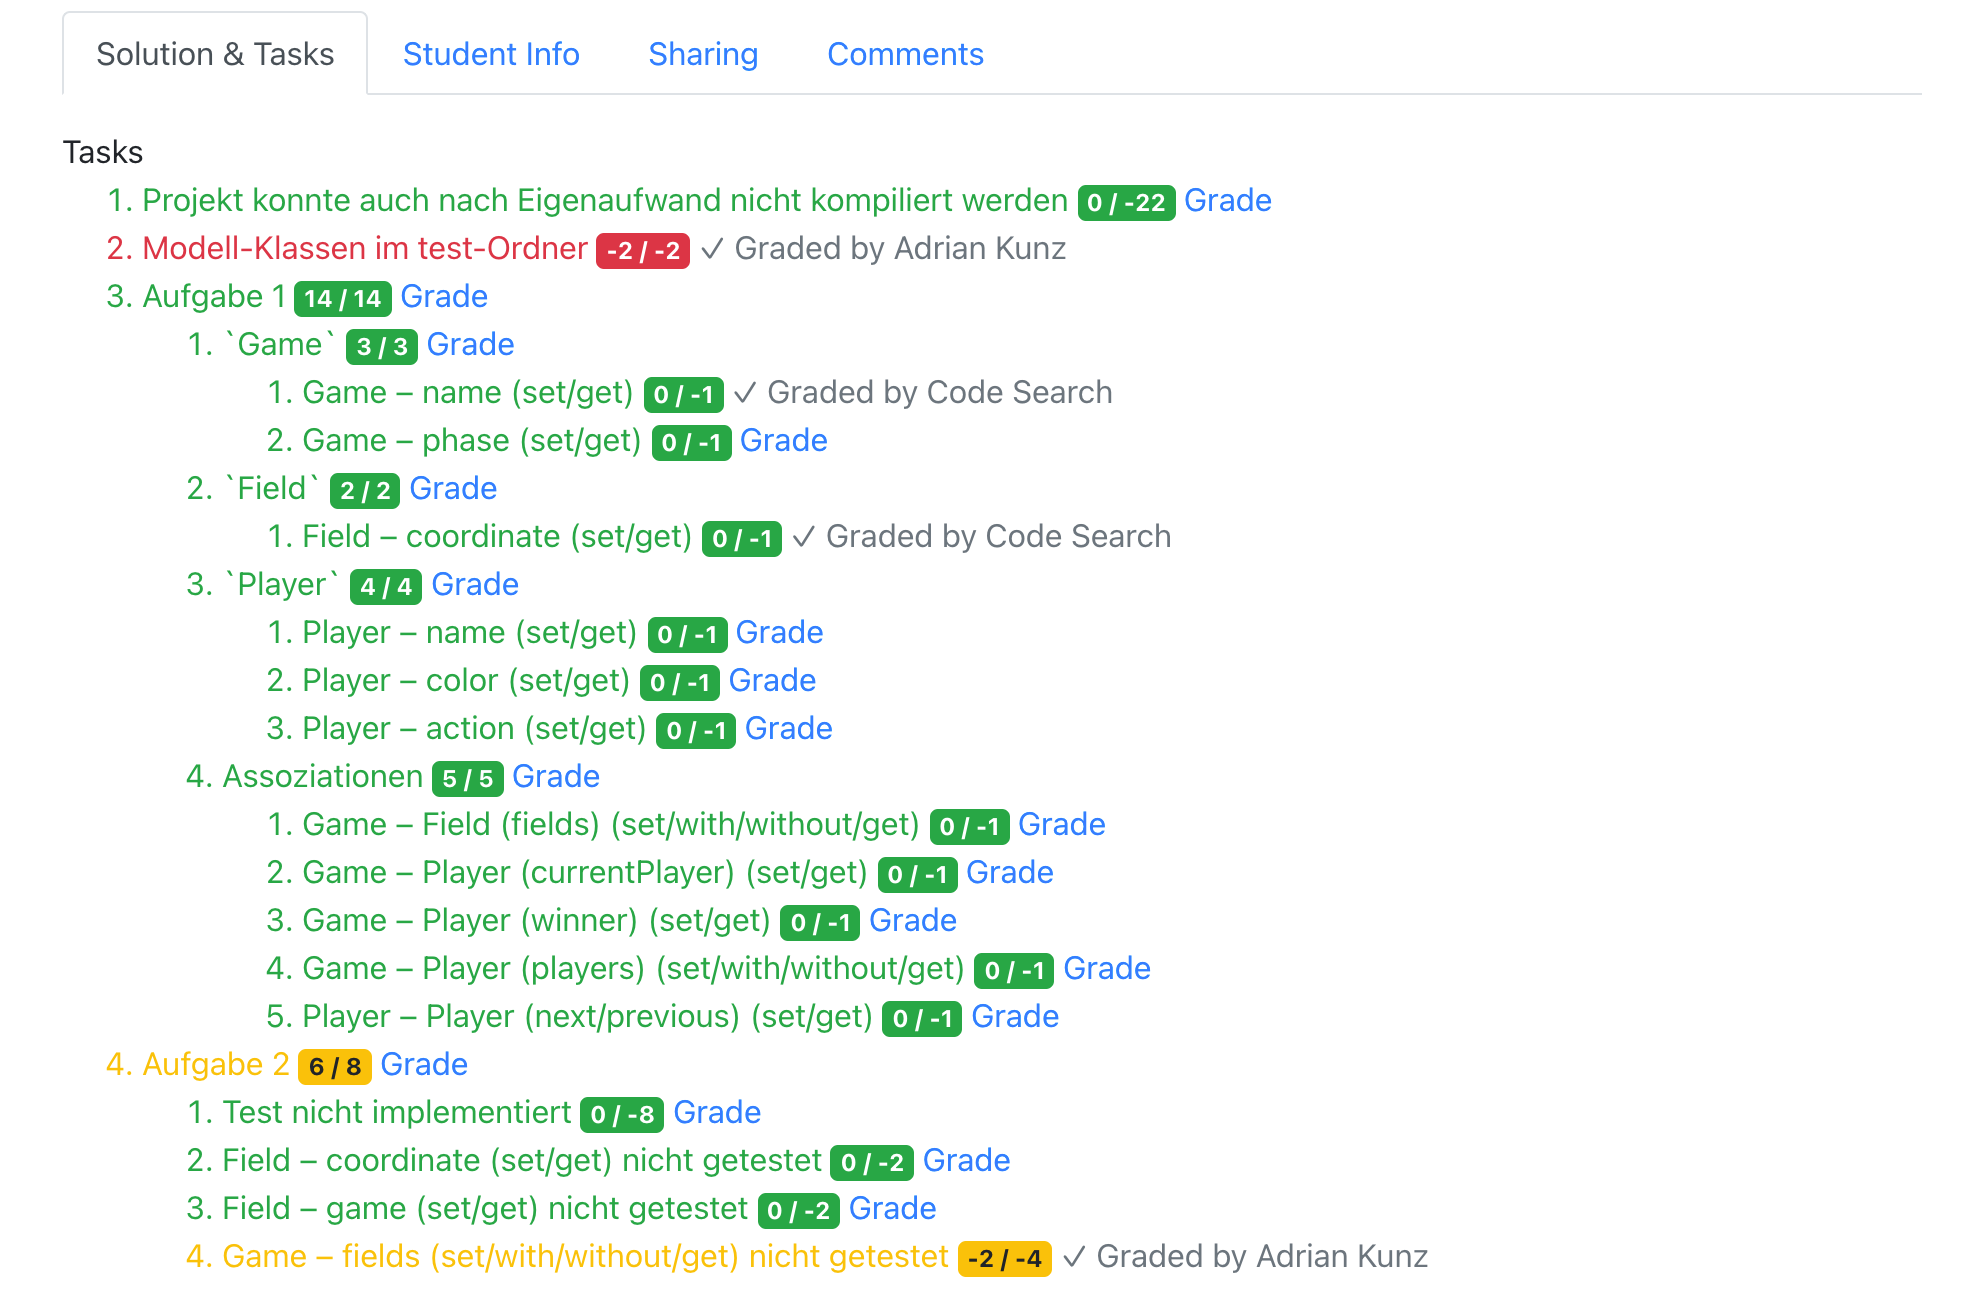
\includegraphics[width=\textwidth]{images/solution-tasks}
    \caption{Teilaufgaben in der Abgabe-Detailansicht}
    \label{fig:solution-tasks}
\end{figure}

Jede Teilaufgabe wird abhängig von der Punktzahl farblich markiert.
Entspricht die vergebene Punktzahl der Minimalpunktzahl eines Tasks, wird dieser rot (\ac{zB} -2/-2).
Werden die maximal mögliche Punkte erreicht, wird der Tasks grün (\ac{zB} 0/-1, 3/3).
Teilpunkte werden gelb dargestellt (\ac{zB} 6/8).
Dabei wird zwischen explizit vergebenen, berechneten und implizit vorhandenen Bewertungen unterschieden.
An der Bezeichnung \textbf{Graded by Name} statt \textbf{Grade} können von Bewertenden vergebene Punktzahlen identifiziert werden.
Teilaufgaben mit eigenen Unteraufgaben berechnen ihre Punktzahl vereinfacht durch Summieren der untergeordneten Punkte\footnote{
    Die genaue Berechnung bezieht Besonderheiten wie Unteraufgaben mit positiver und negativer Punktzahl mit ein.
    Auf die Angabe einer Formel wird an dieser Stelle verzichtet.
}.
Alle anderen Teilaufgaben erhalten standardmäßig null Punkte.
Durch Klicken auf \textbf{Grade} oder \textbf{Graded by Name} kann die Bewertung einer Teilaufgabe angelegt oder bearbeitet werden.
Abbildung~\ref{fig:evaluation-modal} das sich öffnende Modalfenster.

\begin{figure}
    \centering
    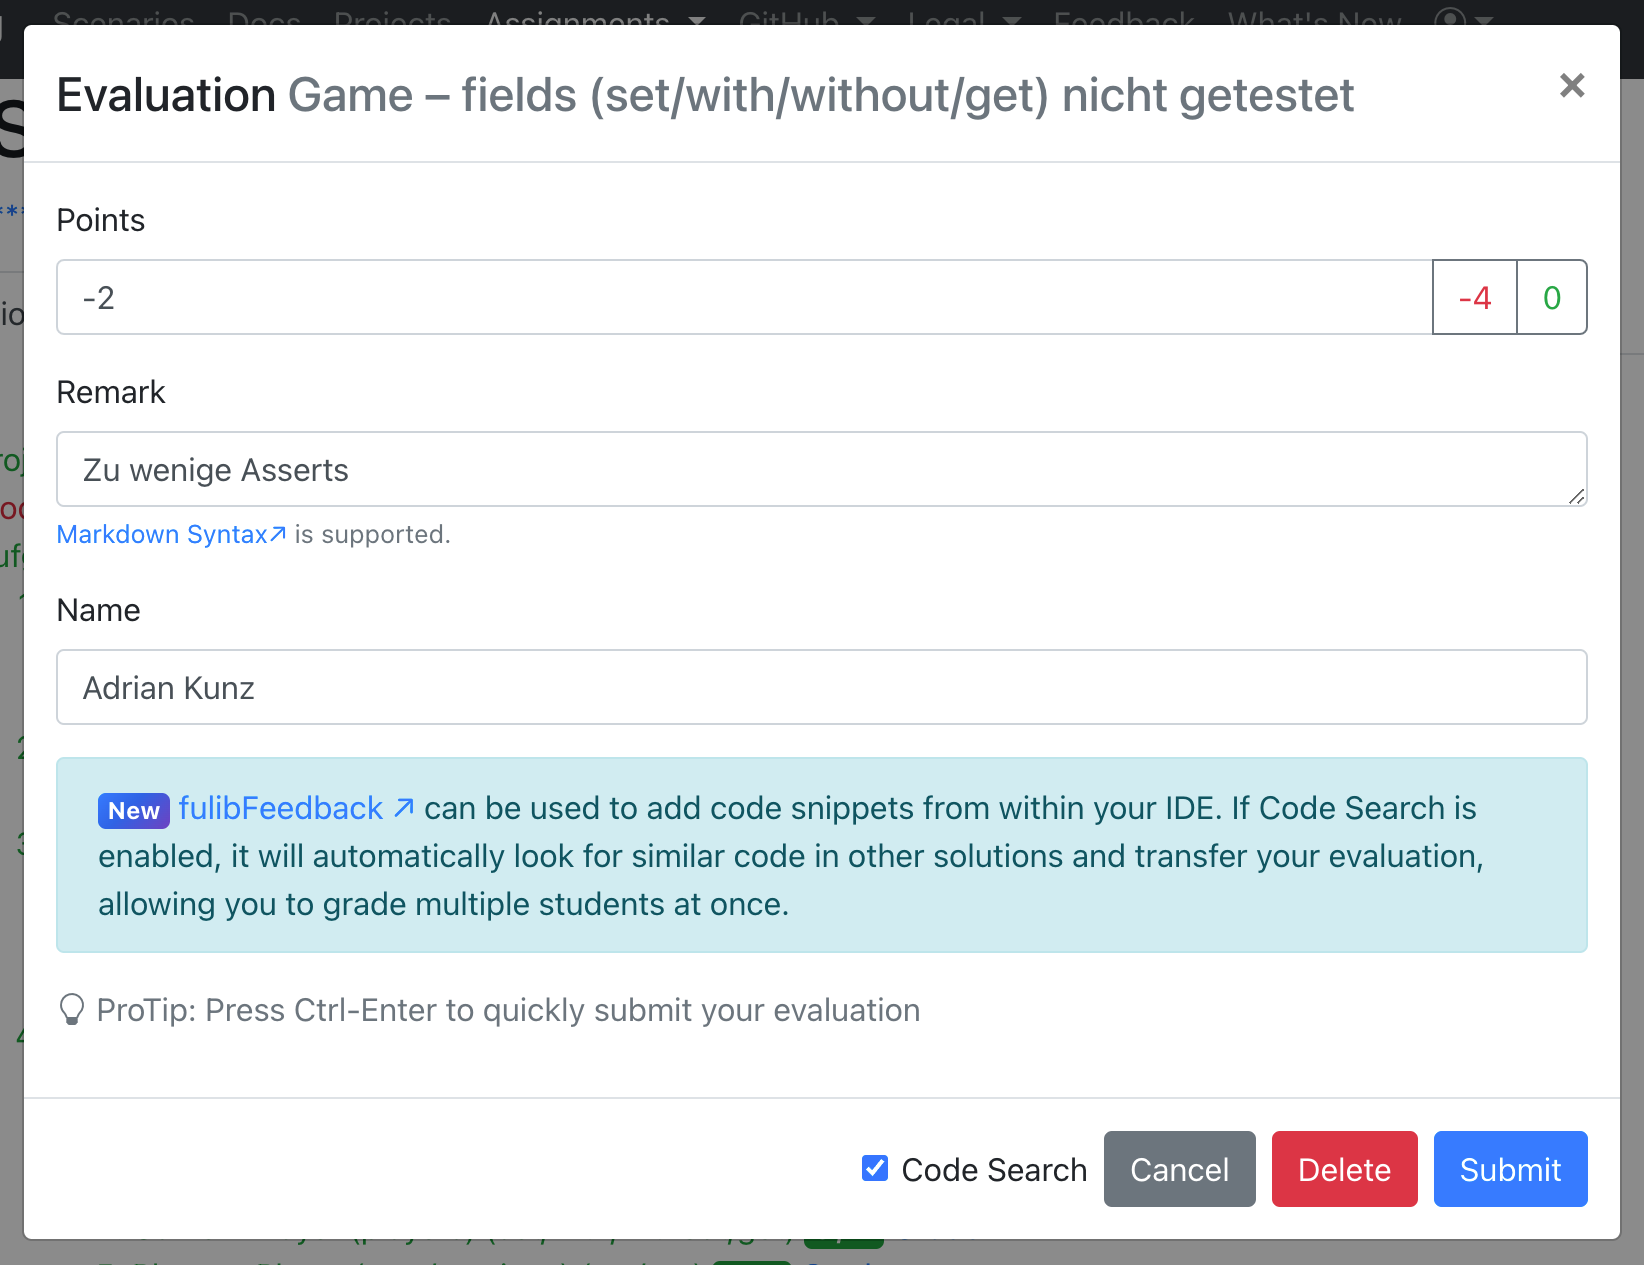
\includegraphics[width=0.8\textwidth]{images/evaluation-modal}
    \caption{Bewertung einer Teilaufgabe}
    \label{fig:evaluation-modal}
\end{figure}

Die Bewertung in dieser Fenster ist zunächst sehr einfach gehalten und für schnelle Bedienbarkeit optimiert.
Im ersten Eingabefeld kann die Punktzahl eingegeben werden oder durch die Kürzelbuttons direkt auf den Minimal- oder Maximalwert gesetzt werden.
Das Feld \textbf{Remark} kann für zusätzliche Hinweise für das Feedback verwendet werden.
Hier kann beispielsweise ein kurzer erklärender Satz oder nach dem Aufklappen zu einem mehrzeiligen Textbereich eine Fehlermeldung eingegeben werden.
Der \textbf{Name} dient der Identifikation des Bewerters, wird aber bei eingeloggten Benutzern oder vorheriger Eingabe automatisch ausgefüllt.
Der Informationstext zu fulibFeedback informiert über dessen Verfügbarkeit zum Hinterlegen von Codebeispielen.
Dies wird in Abschnitt~\ref{sec:fulibFeedback} erneut aufgefasst.
Mit dem \textbf{Submit}-Button wird schließlich die Bewertung gespeichert und das Modalfenster geschlossen.
In Abbildung~\ref{fig:evaluation-modal} wurde eine bereits vorhande Bewertung zum Bearbeiten geöffnet, weshalb der \textbf{Delete}-Button sichtbar ist, um diese zu löschen.

Die Bewertung von Teilaufgaben mit diesem Vorgehen ein wiederkehrender Ablauf, der von Bewertenden hunderte Male pro Hausaufgabe durchgeführt wird.
Daher wurde besonderer Wert darauf gelegt, den Ablauf möglichst effizient zu gestalten.
Während der Bewertung einer Teilaufgabe im Modalfenster wird die Zeit gemessen, die dabei verstrichen ist.
Darauf basierend wird eine Statistik berechnet, welche in Abschnitt~\ref{subsec:statistics} gezeigt und in Kapitel~\ref{ch:evaluation} für einige Realbeispiele ausgewertet wird.

\subsubsection{Feedback}

Der letzte Schritt der Bewertung eines Studierenden ist das Versenden des Feedbacks.
In der Abgabentabelle kann über den zugehörigen Button das Feedback-Modalfenster geöffnet werden, das in Abbildung~\ref{fig:submit-feedback} zu sehen ist.

\begin{figure}
    \centering
    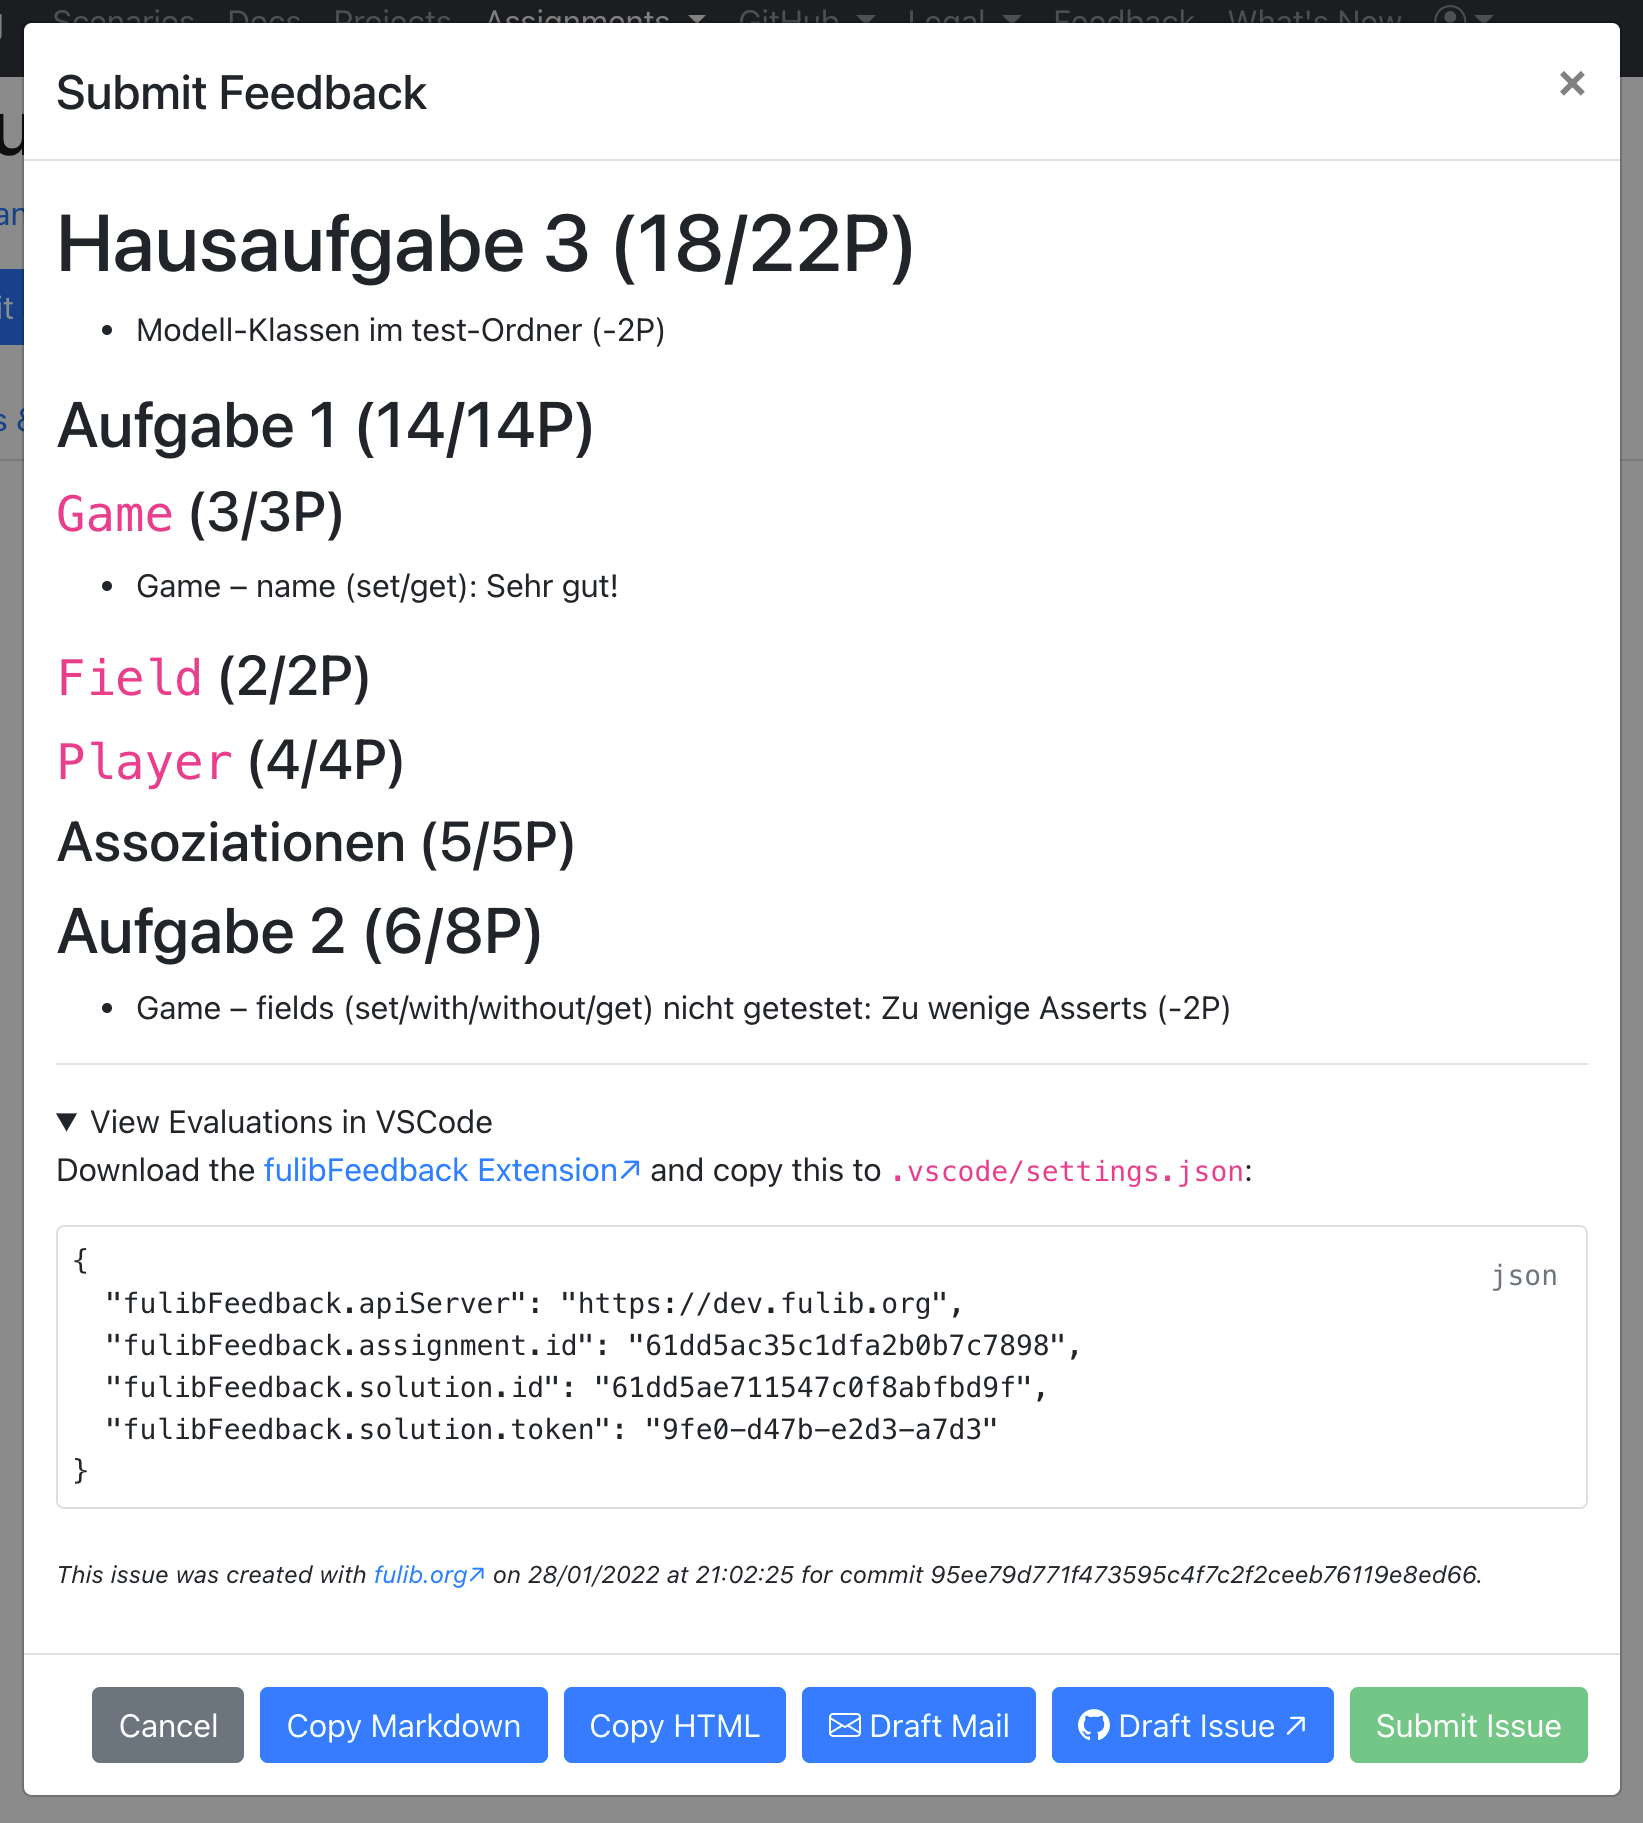
\includegraphics[width=0.8\textwidth]{images/submit-feedback}
    \caption{Modalfenster zum Versenden von Feedback}
    \label{fig:submit-feedback}
\end{figure}

Hier kann nochmal anhand der Vorschau abschließend geprüft werden, ob die Bewertung und Punkteberechnung korrekt durchgeführt wurde.
Daran können nun einige Aspekte der Feedback-Generierung erklärt werden.
Zunächst ist erkennbar, dass nicht jede Teilaufgabe des Assignments hier vertreten ist.
Insbesondere werden Abzüge, \ac{dh} Teilaufgaben mit negativer Punktzahl, nicht angezeigt, sofern sie nicht bewertet wurden.
In seltenen Fällen bietet es sich an, bei diesen Teilaufgaben keine Punkte abzuziehen, aber dennoch ein Kommentar oder eine Hilfestellung in Form des Remarks anzugeben.
Beispiel dafür ist die Teilaufgabe "Game -- name" in Abbildung~\ref{fig:submit-feedback}.
Die Punktzahl wird dann nicht angezeigt, da eine Darstellung wie "(0P)" zu Verwirrung führen könnte.
Teilaufgaben mit positiver Punktzahl werden immer angezeigt.

Am Ende der Bewertung befindet sich stets eine automatisch generierte Fußzeile.
Dort befinden sich Metadaten wie das Bewertungsdatum und der zugrundeliegende Commit.
Die ebenfalls hier aufgeführten fulibFeedback-Einstellungen für \ac{vsc} werden in Abschnitt~\ref{sec:fulibFeedback} erneut erwähnt.

Zum Versenden des Feedbacks werden mehrere Transportwege angeboten.
Mit den Buttons \textbf{Copy Markdown} und \textbf{Copy \acs{html}} kann das Feedback im jeweiligen Textformat in die Zwischenablage kopiert werden.
\textbf{Draft Mail} öffnet das Standard-Mailprogramm des Benutzers und füllt automatisch den Rumpf der Email mit dem Feedback.
Soll die Bewertung über GitHub erfolgen, wie es in diesem Anwendungsbeispiel intendiert ist, gibt es zwei Möglichkeiten des Versands.
Einerseits kann das Formular zum Anlegen eines Issues auf GitHub mit \textbf{Draft Issue} geöffnet werden, sodass ein weiteres Mal der Text überprüft werden kann.
Andererseits kann mit \textbf{Submit Issue} direkt ein Issue über die GitHub \ac{api} und angelegt und somit ein Schritt gespart werden.
In jedem Fall wird die Gesamtpunktzahl, in Abbildung~\ref{fig:submit-feedback} beispielhaft 18/22, für die Abgabe gespeichert, damit sie in der Tabelle mit allen Abgaben angezeigt und die Abgabe eindeutig als bearbeitet erkannt werden kann.
Die Bewertung des Studierenden ist nun abgeschlossen und es kann mit der nächsten fortgefahren werden.

\subsection{Statistiken}\label{subsec:statistics}

Während und nach der Bewertung aller Abgaben können Betreuende und Übungsleitende eine Statistik einsehen.
Sie enthält Informationen über die Anzahl der Bewertungen, die dabei verstrichene Zeit und die Effektivität der automatischen Bewertung von Code Search.
Diese werden sowohl übergreifend als auch pro Teilaufgabe dargestellt.
Zusätzlich wird Einsicht darüber geboten, welche Teilaufgaben am häufigsten zu Punkteeinbußen oder -Abzügen geführt haben.
Daraus lässt sich ableiten, ob Lernziele möglicherweise nicht erreicht werden konnten oder Schwierigkeiten bei der Umsetzung bestanden.

Die Statistik kann in der Assignment-Übersicht unter dem gleichbenannten Tab gefunden werden.
In Abbildung~\ref{fig:assignment-statistics-basics} sind zunächst die übergreifenden Informationen dargestellt.
Die Seite gliedert sich in drei Abschnitte, \textbf{Solutions}, \textbf{Evaluations} und \textbf{Time Tracking}.

\begin{figure}
    \centering
    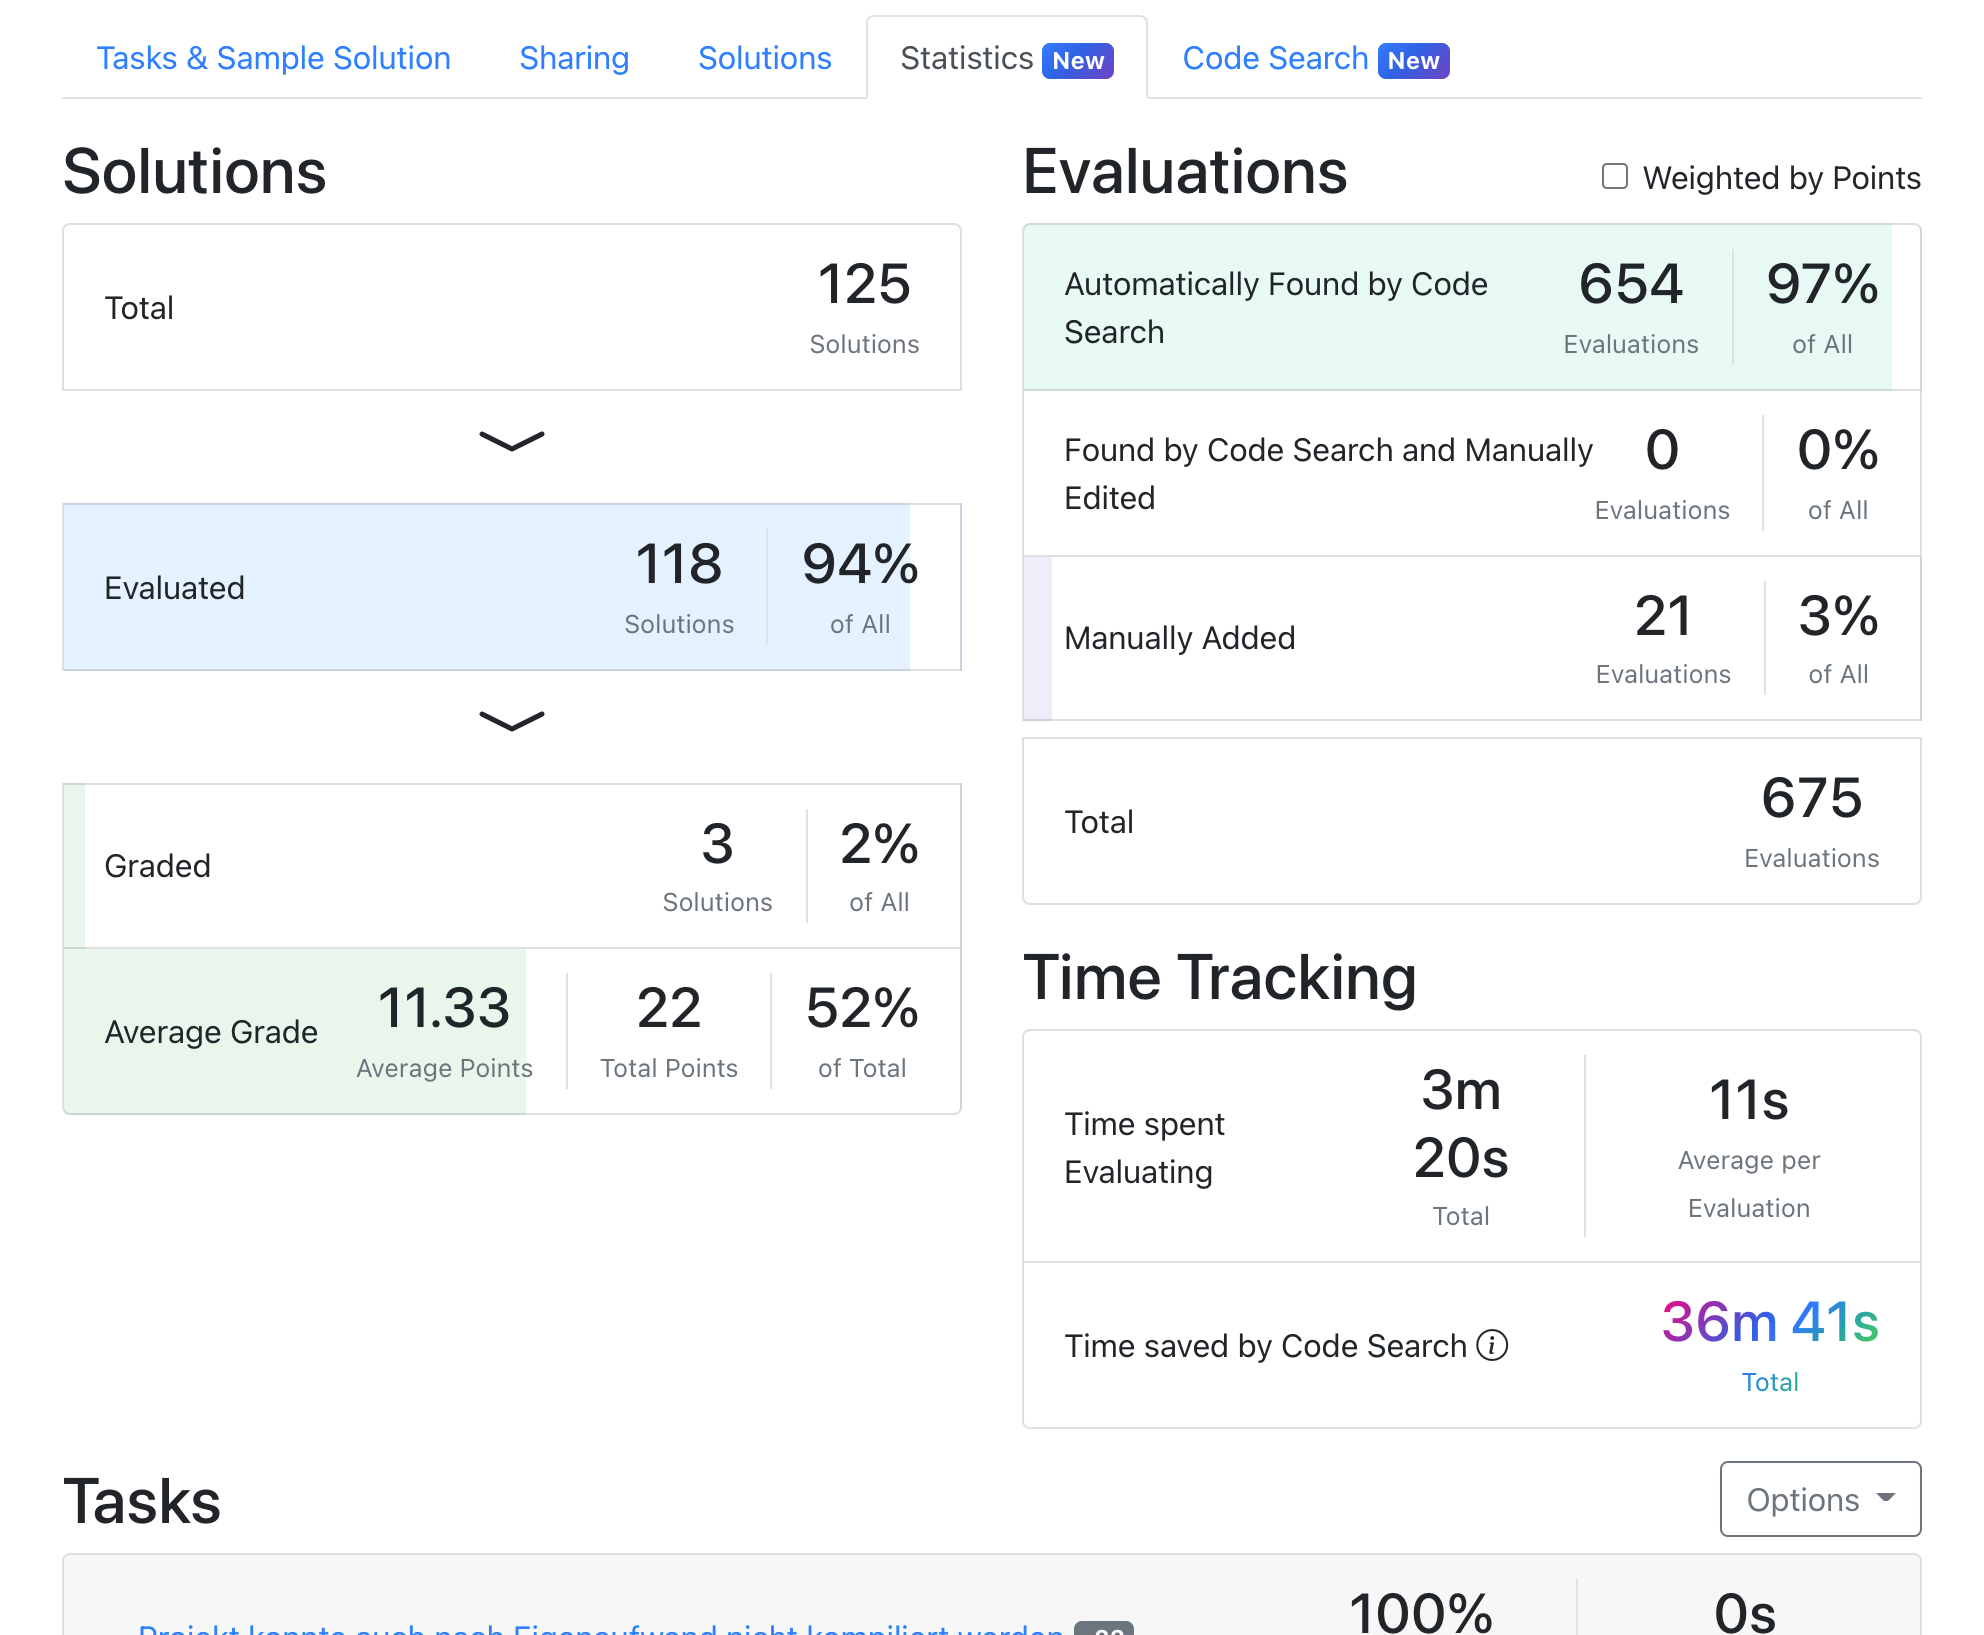
\includegraphics[width=\textwidth]{images/assignment-statistics-basics}
    \caption{Übergreifende Statistiken}
    \label{fig:assignment-statistics-basics}
\end{figure}

Unter Solutions ist jeweils die Anzahl der Abgaben insgesamt (\textbf{Total}), mit angefangener Bewertung (\textbf{Evaluated}) und mit versendeten Feedback abgeschlossenen (\textbf{Graded}) sichtbar.
Zudem wird die durchschnittlich erreichte Punktzahl der abgeschlossenen Abgaben abgezeigt\footnote{
    Es handelt sich bei diesem und folgenden Screenshots der Statistik nicht um die realen Zahlen der Hausaufgabe 3.
}.

Die Evaluations\footnote{
    Bewertungen von Teilaufgaben.
} werden für die Auswertung in drei Kategorien unterteilt.
Händisch hinzugefügte Bewertungen sind genau diejenigen, die wie in Abschnitt~\ref{subsec:grading} beschrieben erstellt wurden.
Von Code Search gefundene Bewertungen können anhand der vorherigen erstellt werden und geben Aufschluss darüber, wie effektiv das Werkzeug für die vorliegende Hausaufgabe war.
In seltenen Fällen ist es notwendig, diese automatisch erstellten Bewertungen händisch anzupassen, wenn beispielsweise eine Suche zu ungeeigneten Ergebnisse geführt hat.
Diese Fehlerfälle sowie die sich ergebenden relativen Anteile der Kategorien werden in Kapitel~\ref{ch:evaluation} näher erläutert und diskutiert.

Der Abschnitt Time Tracking dient der Berechnung der Effizienz von Bewertenden und Code Search.
Anhand der Zeitmessung, die während der Bewertung von Teilaufgaben stattfindet, können hier eine Gesamtdauer und der Durchschnitt pro Teilaufgabe berechnet werden.
Weiterhin wird hier angezeigt, wie viel Zeit durch die Verwendung von Code Search eingespart werden konnte.
Die Berechnung dieses Werts erfordert die Betrachtung der Teilaufgaben und wird in Kürze erläutert.
Kapitel~\ref{ch:evaluation} wird diesen Messwert anhand einiger realer Beispiele verwenden, um die Effizienz von Code Search zu bestimmen.

\begin{figure}
    \centering
    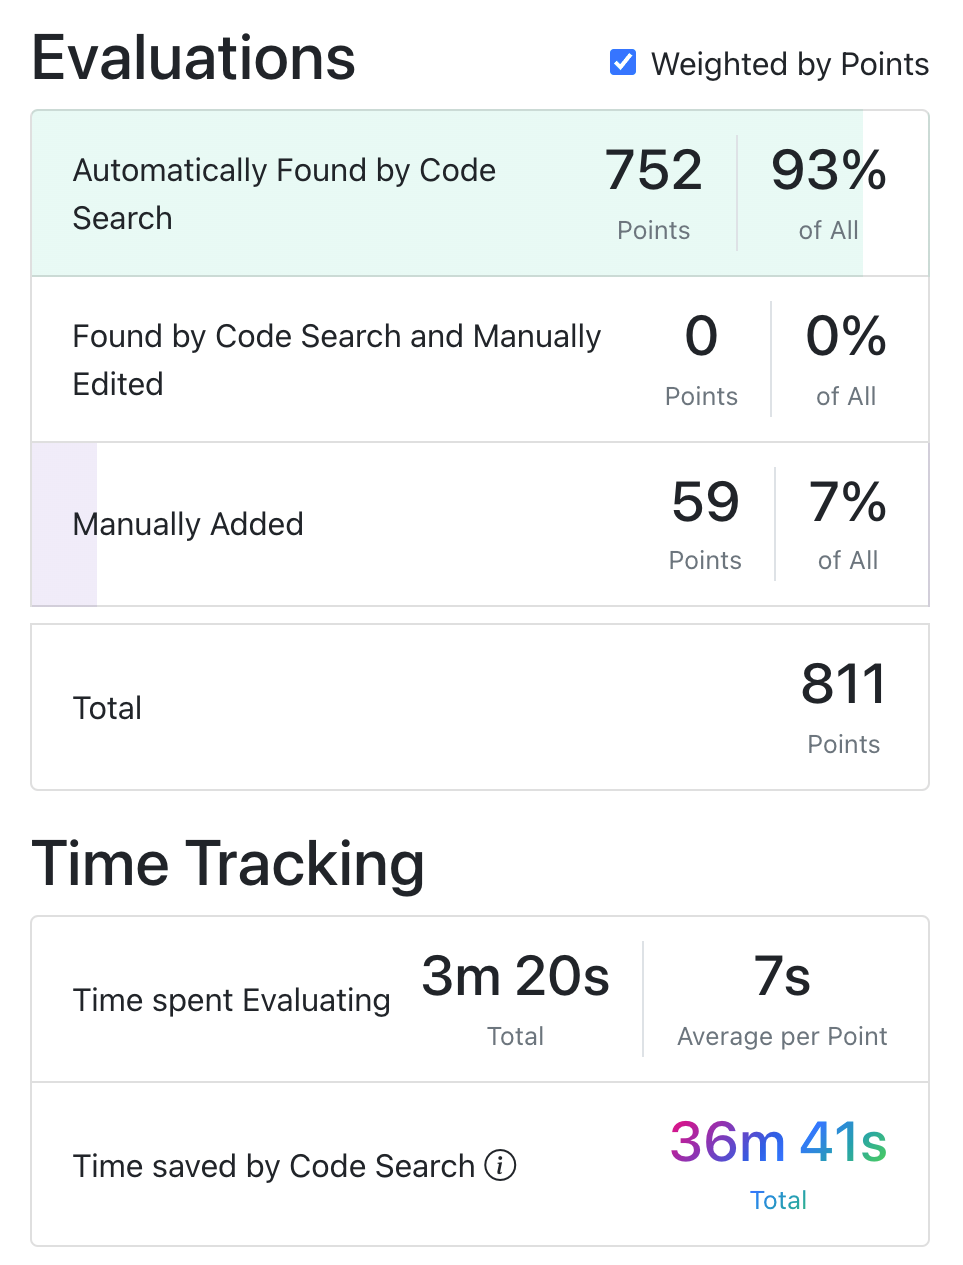
\includegraphics[width=0.5\textwidth]{images/assignment-statistics-by-points}
    \caption{Statistiken gewichtet nach Punkten}
    \label{fig:assignment-statistics-by-points}
\end{figure}

Evaluations und Time Tracking können die Ansicht verändern, um Punktzahlen statt Bewertungen von Teilaufgaben als Bewertungsgrundlage zu verwenden.
Dafür wird der Haken \textbf{Weighted by Points} gesetzt, wie Abbildung~\ref{fig:assignment-statistics-by-points} zeigt.
Dadurch kann ein Vergleich zwischen Bewertungs-Einheiten und Punkteeinheiten erfolgen und ermittelt werden, in welcher Relation der Arbeitsaufwand und die vergebeben Punkte stehen.
Dies ist besonders dann interessant, wenn die Punkte direkten Einfluss auf die Benotung der Veranstaltung haben, wie es bei Laborveranstaltungen der Fall sein kann.
In Kapitel~\ref{ch:evaluation} werden einige Beispiele betrachtet, wo die Punktzahl und Bewertungsanzahl teilweise stark unterschiedlich sind, wenn Teilaufgaben mit mehr als einem Punkt bewertet werden.

\begin{figure}
    \centering
    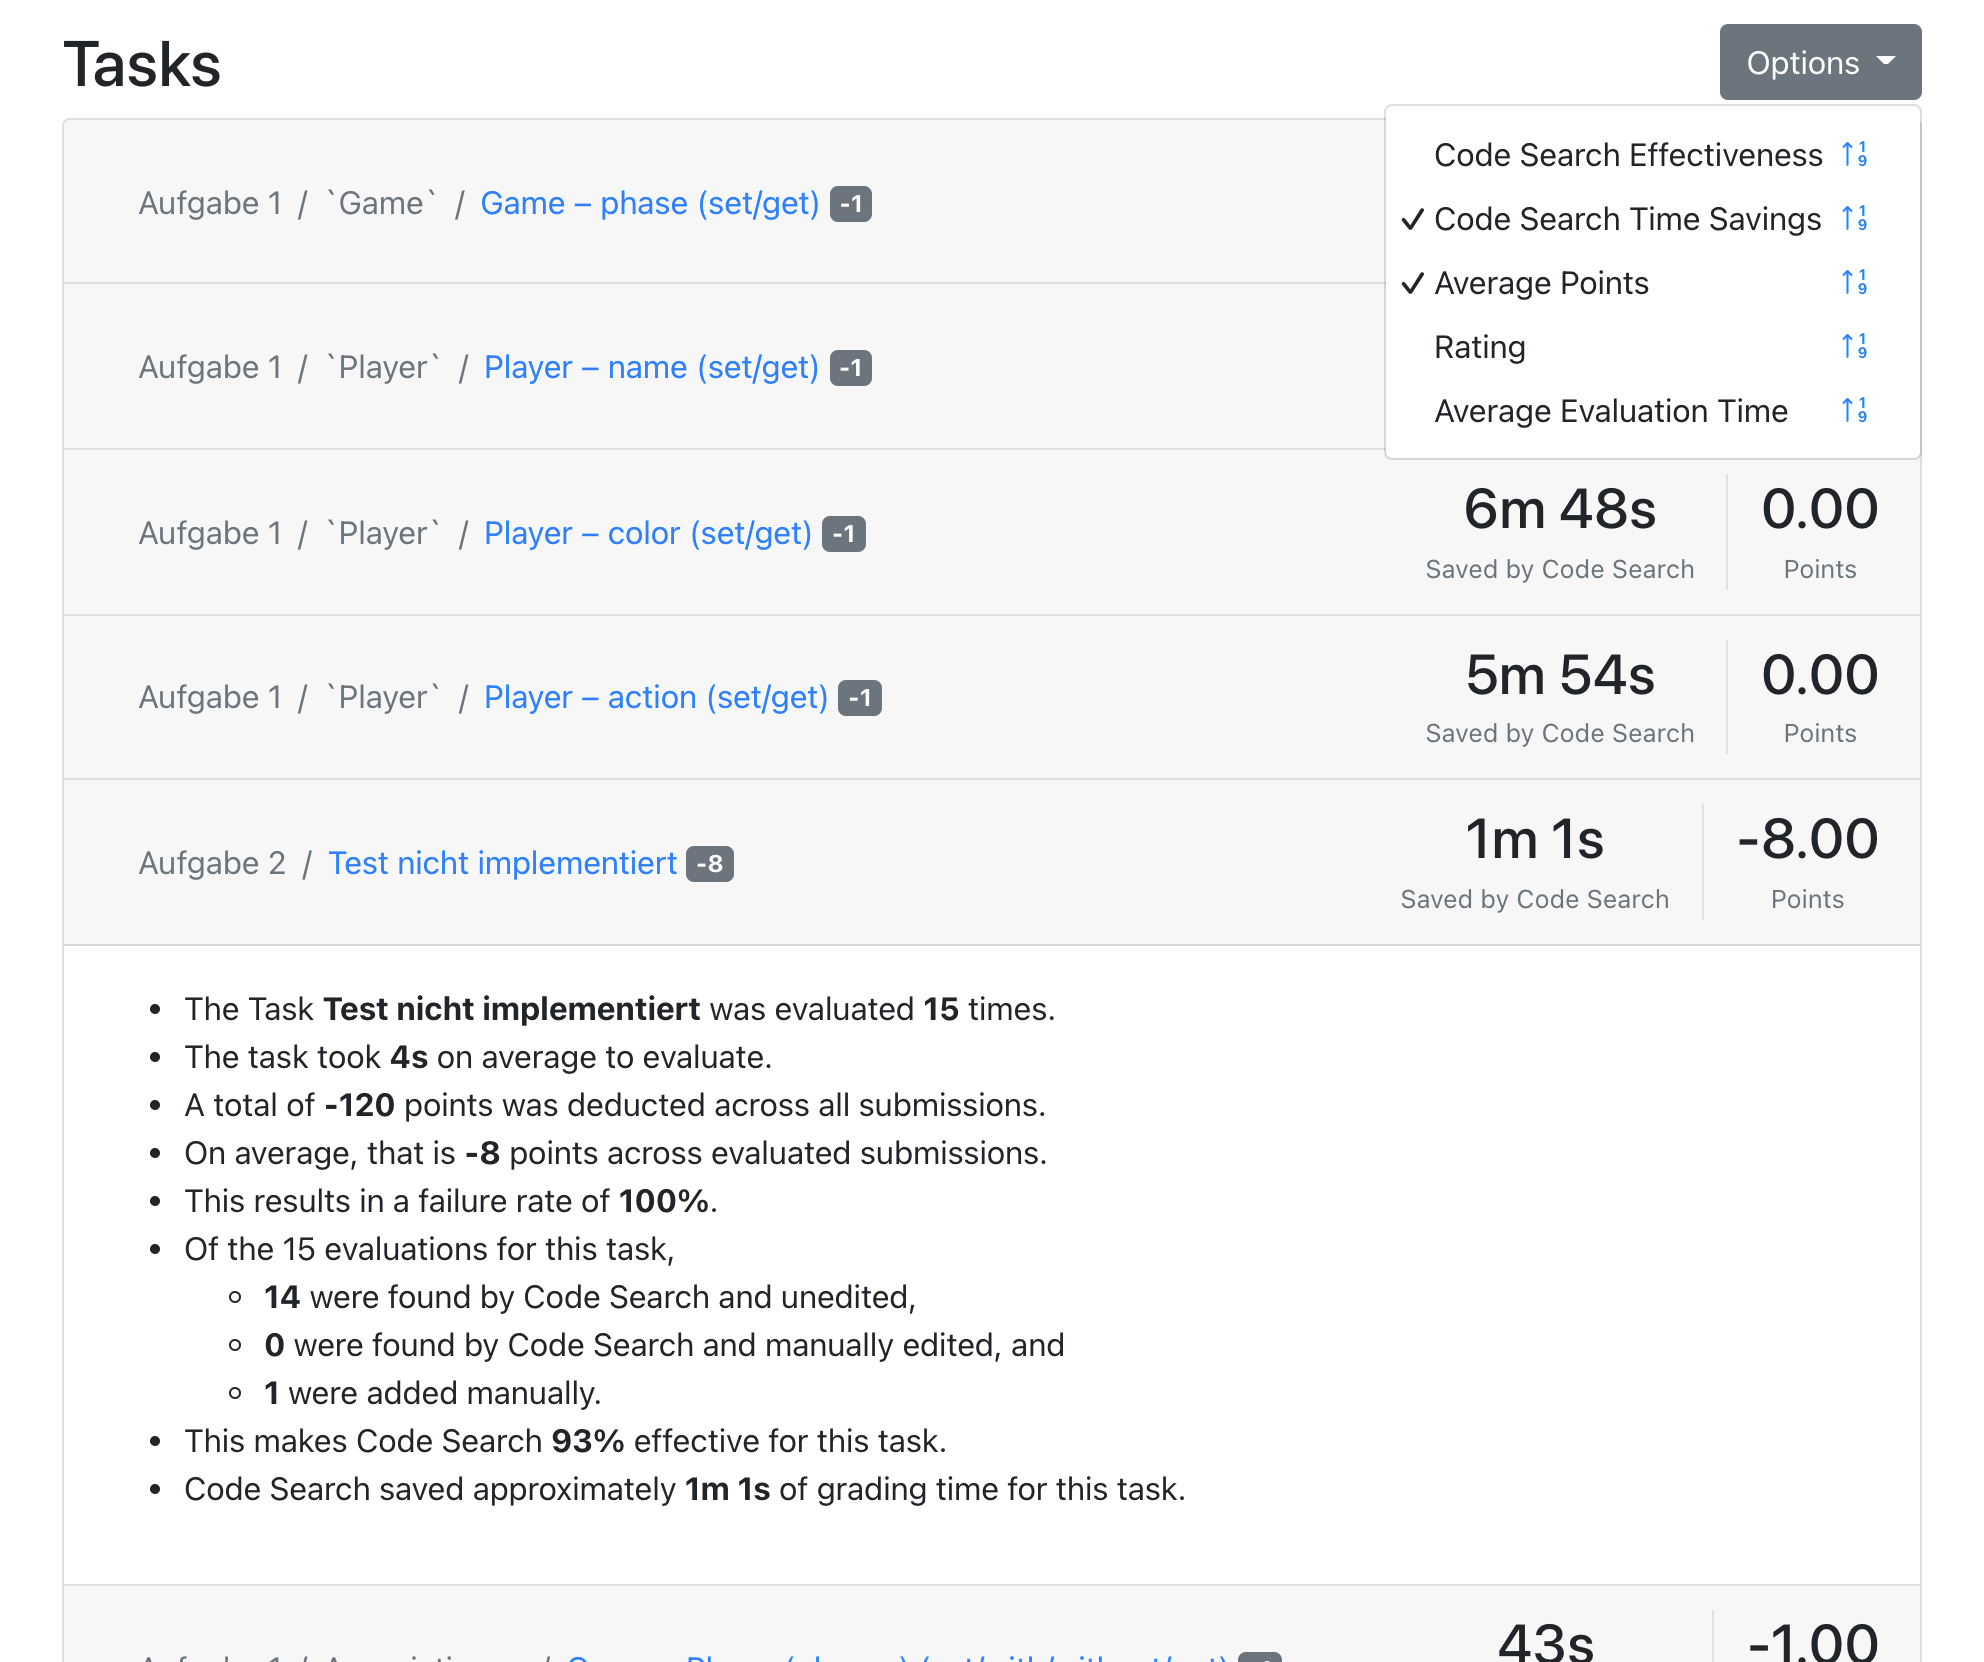
\includegraphics[width=\textwidth]{images/assignment-statistics-tasks.png}
    \caption{Statistiken für einzelne Teilaufgaben}
    \label{fig:assignment-statistics-tasks}
\end{figure}

Im unteren Teil der Statistik befindet sich eine Liste aller Teilaufgaben, wie Abbildung~\ref{fig:assignment-statistics-tasks} zeigt.
Die Informationen in der Kopfzeile jedes Eintrags sind mit dem Options-Menü auswählbar.
Dort kann zwischen den wichtigsten Metriken ausgewählt werden.
Diese werden nachfolgend kurz beschrieben.
Zudem kann die Liste anhand der Werte auf- oder absteigend sortiert werden.
Jeder Eintrag kann individuell ausgeklappt werden, um weitere Details anzuzeigen.
Dafür werden jeweils kurze Stichpunkte zu jedem Wert genannt, um Hinweise auf dessen Bedeutung zu geben.

\begin{description}
    \item[Code Search Effektiveness] ist der Anteil der Bewertungen für diese Teilaufgabe, die automatisch von Code Search angelegt wurden.
    Im Beispiel der Teilaufgabe \textbf{Aufgabe 2 / Test nicht implementiert} wurde eine Bewertung händisch angelegt und auf 14 weitere Abgaben von Code Search kopiert.
    Dies ergibt eine Effektivität von $\frac{14}{1 + 14} = \frac{14}{15} \approx 93\%$.\footnote{
        Die Effektivität kann nie 100\% betragen, da Code Search nur ausgehend von einer händischen Bewertung aktiviert wird.
        Beim Löschen von dieser werden auch davon abstammende Code Search-Bewertungen gelöscht.
    }
    \item[Average Evaluation Item] ist die durchschnittliche Bewertungsdauer der Teilaufgabe.
    Diese wird gemessen, während das Bewertungs-Modalfenster geöffnet ist.
    Das verlängertes Öffnen dieses Fensters, beispielsweise beim Verlassen des Arbeitsplatzes oder beim Einlegen einer Pause, kann die Statistik verfälschen.
    Um dies zu vermeiden, werden Ausreißer länger als 60 Sekunden nicht im Durchschnitt verrechnet.
    \item[Code Search Time Savings] bezeichnet die geschätze Zeit, die durch Code Search bei der Bewertung dieser Teilaufgabe eingespart wurde.
    Sie berechnet sich durch Multiplikation der Average Evaluation Time mit der Anzahl der von Code Search erstellten Bewertungen.
    Die Summe dieser Werte über alle Teilaufgaben ergibt die zuvor genannte Zeit, die insgesamt mit Code Search gespart wurde.
    \item[Average Points] ist die durchschnittlich vergebene Punktzahl über alle Bewertungen dieser Teilaufgabe.
    \item[Rating] ergibt sich aus den Average Points geteilt durch die maximal erreichbare Punktzahl der Teilaufgabe.
    Dadurch ergibt sich eine relative Prozentangabe, die mit anderen Teilaufgaben verglichen werden kann.
    Mit diesem Wert können insbesondere die Teilaufgaben identifiziert werden, die am häufigsten zu Punktabzug geführt haben und mögliche Problemquellen für Studierende darstellen.
\end{description}

\subsection{Code Search}\label{subsec:code-search}

Wie zuvor erwähnt handelt es sich bei Code Search um eine Suchmaschine für Quellcode in Assignments.
Es gibt zwei Wege diese zu aktivieren.
Einerseits kann der dafür vorgesehene Tab in der Assignment-Übersicht verwendet werden, der in Abbildung~\ref{fig:assignment-code-search} dargestellt ist.
Andererseits wird Code Search verwendet, um automatisch Bewertungen von Teilaufgaben anhand von ausgewählten Codeschnipseln zu erstellen.
Dies wird in Abschnitt~\ref{sec:fulibFeedback} detailliert beschrieben.
Zunächst wird nur der Such-Tab erläutert, um einen Einblick in die Hintergründe der Suchmaschine zu bieten.

\begin{figure}
    \centering
    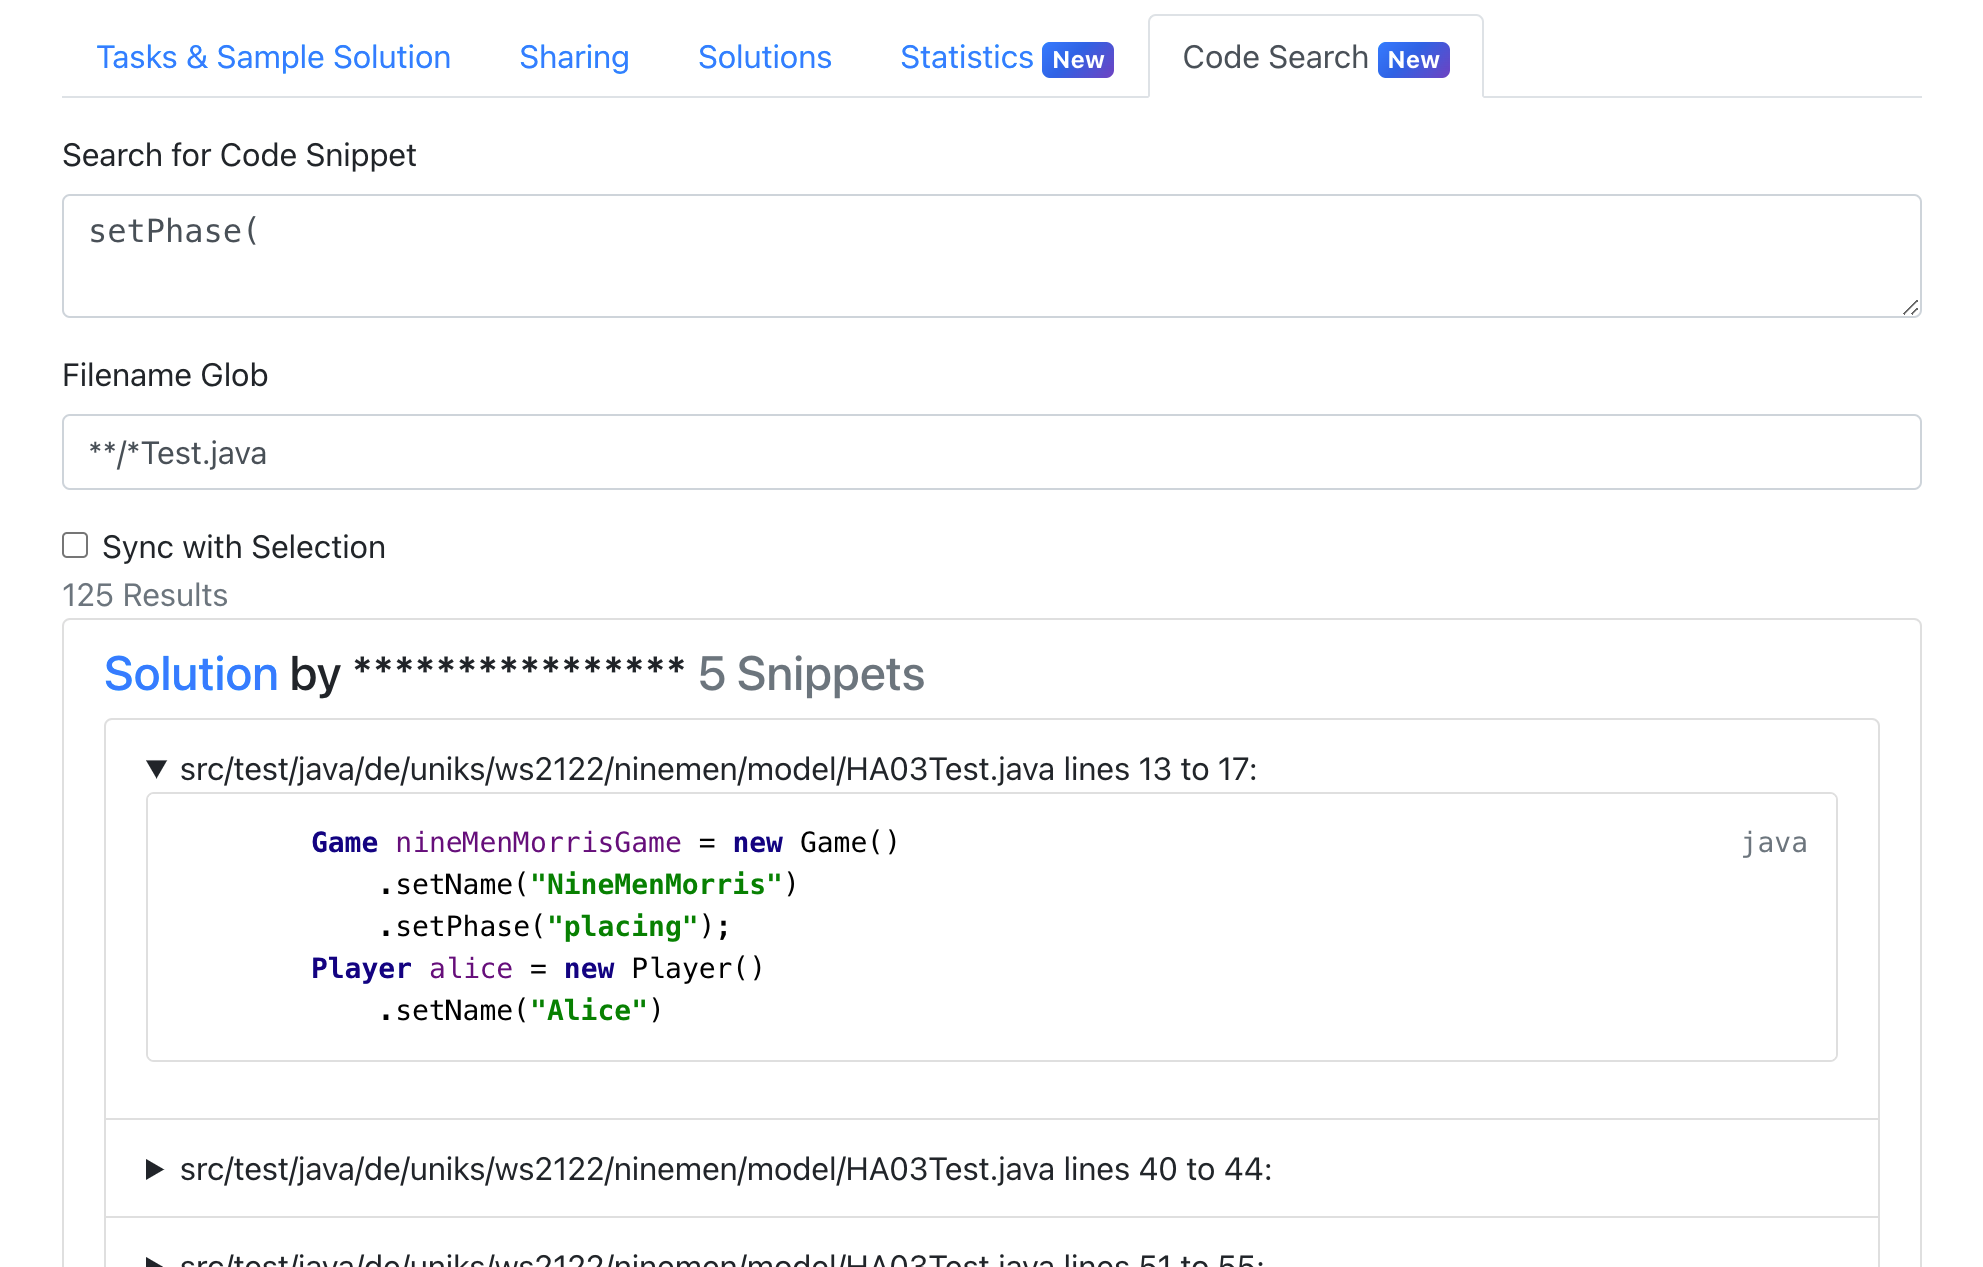
\includegraphics[width=\textwidth]{images/assignment-code-search.png}
    \caption{Code Search Tab eines Assignments}
    \label{fig:assignment-code-search}
\end{figure}

Die wichtigste Eingabe auf diesem Tab ist das \textbf{Code Snippet}, welches die Suchanfrage bildet.
Diese wird an die Elasticsearch-Datenbank, welche beim Import von Lösungen mit deren Dateien gefüllt wurde, gestellt.
Die Datenbank gibt als Ergebnis der Suchanfrage alle Dateien zurück, welche diesen Codeabschnitt beinhalten.
Insbesondere ist dabei die Formatierung des Codes unerheblich:
die Suche arbeitet anhand von Tokens, wie in Abschnitt~\ref{subsec:elasticsearch} beschrieben wurde.
Da es sich nicht um natürlichsprachliche Texte handelt, für die Elasticsearch standardmäßig konfiguriert ist, muss zunächst eine angepasster Tokeniser definiert werden.
Dieser besteht hauptsächlich aus einem regulären Ausdruck, der Tokens erkennt.
Listing~\ref{lst:code-search-regex-builder} zeigt den TypeScript-Code, der diesen regulären Ausdruck konstruiert.

\begin{listing}
    \centering
    \begin{minted}{ts}
        const pattern = Object.values({
            number: /[+-]?[0-9]+(\.[0-9]+)?/,
            string: /["](\\\\|\\["]|[^"])*["]/,
            char: /'(\\\\|\\'|[^'])*'/,
            identifier: /[a-zA-Z$_][a-zA-Z0-9$_]*/,
            symbol: /[(){}<>\[\].,;+\-*/%|&=!?:@^]/,
        }).map(r => r.source).join('|');
    \end{minted}
    \caption{Konstruktion des regulären Ausdrucks für Tokens}
    \label{lst:code-search-regex-builder}
\end{listing}

Die verschiedenen Arten von Tokens (Zahlen, String-Literale mit einfachen und doppelten Anführungsstrichen, Bezeichner und Symbole) werden als separate reguläre Ausdrücke definiert und dann mit Alternations-Symbolen (\texttt{|}) getrennt konkateniert.
Es wird an dieser Stelle auf genauere Beschreibung der regulären Ausdrücke verzichtet.
Entscheidend ist nur, dass diese gewählt wurden, um für möglichst viele Programmiersprachen sinnvolle Tokens zu erzeugen.
Die Syntax für Zahlen, String-Literale, Bezeichner und Symbole orientiert sich an populären\footnote{
    \url{https://www.tiobe.com/tiobe-index/}
} Programmiersprachen wie Java, JavaScript, C und Python.

Der \textbf{Filename Glob} dient der Einschränkung der Suche auf bestimmte Dateien.
Dafür wird die spezielle Glob-Syntax\footnote{
    \url{https://en.wikipedia.org/wiki/Glob_(programming)}
} verwendet, welche die Verwendung von Platzhaltern erlaubt.
Das Beispiel \texttt{**/*Test.java} aus Abbildung~\ref{fig:assignment-code-search} wählt nur Dateien aus, die auf \texttt{Test.java} enden (\texttt{*Test.java}) und sich in einem beliebigen Unterordner des Projekts befinden (\texttt{**/}).
Für die Suche mit Elasticsearch wird das Glob-Muster in einen regulären Ausdruck übersetzt und als Filterbedingung in der Suchanfrage an die Datenbank übergeben.

Alle Suchergebnisse werden gruppiert nach Abgabe in einer Liste angezeigt.
Neben dem Dateinamen werden jeweils die Zeilennummern angegeben, in denen der Code gefunden wurde.
Eine Vorschau zeigt zentral die Zeile mit dem Codeabschnitt und davor und danach zwei Zeilen des umliegenden Codes als Kontext.
Zeilennummern und Kontext werden nicht von Elasticsearch in den Suchergebnissen bereitgestellt.
Anhand des in Abschnitt~\ref{subsec:elasticsearch} beschriebenen Highlighters wird stattdessen die Stelle im Quelltext markiert, wo der Codeabschnitt gefunden wurde.
Daraus werden Zeilennummern und Kontext rekonstruiert.

Die Aufgabe des Code Search-Tabs ist insbesondere die Vorschau für die mögliche automatische Bewertung mit fulibFeedback.
Die Auswahl \textbf{Sync with Selection} aktiviert die Synchronisation des Code Snippets mit fulibFeedback und wird im folgenden Abschnitt beschrieben.
Ebenso kann dieser eingesetzt werden, um bei Verdacht Plagiate zwischen Lösungen zu finden.

\section{fulibFeedback}\label{sec:fulibFeedback}

Die Bewertung von Quellcode auf fulib.org ist zwar möglich, kann aber toolgestützt noch verbessert werden.
Dafür wurde die \ac{vsc}-Erweiterung fulibFeedback entwickelt, die in diesem Abschnitt vorgestellt wird.
Die Erweiterung hat nur eine geringfügige Oberfläche und ist hauptsächlich im Hintergrund tätig.
Nachfolgend wird die Benutzung in der Reihenfolge beschrieben, wie sie für Betreuende und Studierenden chronologisch abläuft.

\subsection{Installation}

Zunächst muss die Erweiterung installiert werden.
Dies ist über den Visual Studio Marketplace\footnote{
    \url{https://marketplace.visualstudio.com/items?itemName=fulib.fulibFeedback}
} möglich.
Ein einfacher Klick auf \textbf{Install} genügt, um zur \ac{vsc}-Anwendung zu wechseln und die Erweiterung hinzuzufügen.

\subsection{Einrichtung}

\begin{figure}
    \centering
    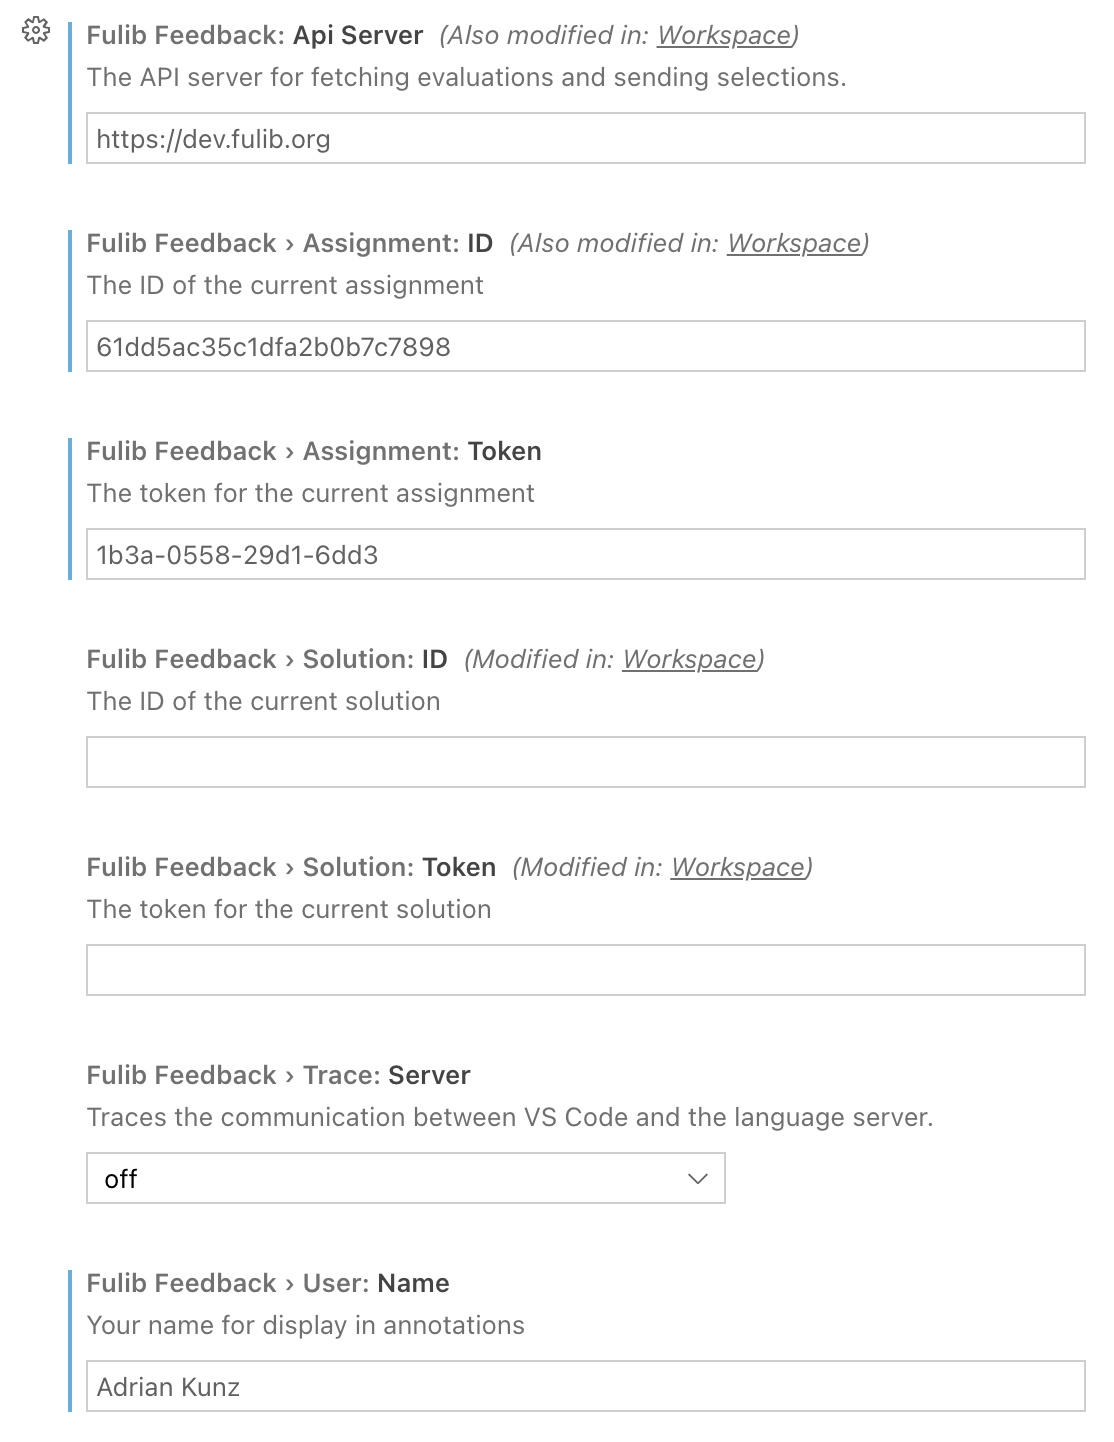
\includegraphics[width=0.55\textwidth]{images/fulibFeedback-settings.png}
    \caption{Einstellungen von fulibFeedback}
    \label{fig:fulibFeedback-settings}
\end{figure}

Um die Erweiterung einzurichten, müssen zunächst einige Einstellungen getätigt werden.
Abbildung~\ref{fig:fulibFeedback-settings} zeigt den Abschnitt von fulibFeedback in den Einstellungen von \ac{vsc}.
Einmalig müssen Bewertende hier ihren Namen unter \textbf{User Name} eingeben.
Dies dient der Zuordnung von ausgewählten Codeabschnitten im weiteren Verlauf.
Für jede Hausaufgabe müssen gegeben ein Assignment dessen \textbf{\acs{id}} und \textbf{Token} angegeben werden.
Studierende haben nicht das Token des Assignments, dafür jedoch eine Solution mit einer \textbf{\acs{id}} und zugehörigem \textbf{Token}.
Der \textbf{\acs{api} Server} kann für Entwicklungszwecke geändert werden.

Um die Einrichtung zu beschleunigen, müssen diese Einstellung \ac{idR} nicht von Hand getätigt werden.
Es genügt, die \textbf{Configure}-Buttons unter den \textbf{Sharing}-Tabs von Assignment\footnote{
    Siehe Abbildung~\ref{fig:assignment-share}.
} oder Solution\footnote{
    \todo{Keine Abbildung?}
} zu drücken.
Sämtliche relevante Einstellungen mit Ausnahme des Namens verwenden dann automatisch ausgefüllt.
Dabei wird auch zwischen globalen Einstellungen und Workspace\footnote{
    Bezeichnet den aktuell geöffneten Projektordner.
}-spezifischen unterschieden.
Assignment-Einstellungen werden automatisch global hinterlegt, um beim Öffnen weiterer Lösungen erhalten zu bleiben.
Solution-Einstellungen werden lediglich im Workspace abgelegt, da sie nur für diese gültig sind.

Wird ein Projektordner geöffnet, versucht die Erweiterung, diesen einer Solution zuzuordnen.
Wurde in den Einstellungen eine Solution \acs{id} angegeben, sind keine weiteren Schritte notwendig.
Anderfalls wird der Pfad der zuerst geöffnet Datei betrachtet und wie in~\ref{eqn:absolute-path-deconstruction} dekonstruiert.

\begin{equation}\label{eqn:absolute-path-deconstruction}
    \text{/Users/\dots/}
    \underbrace{\text{pmws2122-assignment-3}}_{\text{Präfix}}
    \text{-}
    \underbrace{\text{********}}_{\text{GitHub-Name}}
    \text{/}
    \underbrace{\text{src/\dots/Field.java}}_{\text{Relativer Pfad}}
\end{equation}

Damit das Präfix gefunden werden kann, müssen anhand der eingestellten \acs{id} das Assignment und dessen Classroom Prefix ermittelt werden.
Anderfalls kann auch der GitHub-Name und der relative Pfad nicht bestimmt werden.
Bei erfolgreicher Bestimmung der Lösung wird eine Hinweismeldung angezeigt, die in Abbildung~\ref{fig:fulibFeedback-notification} dargestellt ist und Auskunft über den Titel des Assignments und den Namen des Studierenden gibt.

\begin{figure}[h]
    \centering
    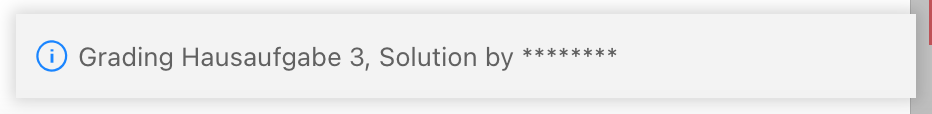
\includegraphics[width=0.45\textwidth]{images/fulibFeedback-notification}
    \caption{Benachrichtigung nach erfolgreicher Ermittlung von Asssignment und Solution}
    \label{fig:fulibFeedback-notification}
\end{figure}

\subsection{Auswahl von Codeabschnitten}

Die wichtigste Funktion von fulibFeedback für Bewertende ist die Auswahl von Codeabschnitten.
Auswahl bezeichnet hier die Aktion, die mit Maus oder Tastatur in gewöhnlichen Texteditoren durchgeführt wird, um beispielsweise Text zum Kopieren zu markieren.
fulibFeedback erkennt dies und sendet den ausgewählten Code zusammen mit Kontextdaten wie Assignment, Solution, Datei und Zeilen- und Spaltennummern an den Backend-Dienst von fulib.org.
Wurde auf fulib.org zuvor ein Bewertungs-Modalfenster für die gleiche Abgabe geöffnet, wird der ausgewählte Code dort angezeigt.

\begin{figure}
    \centering
    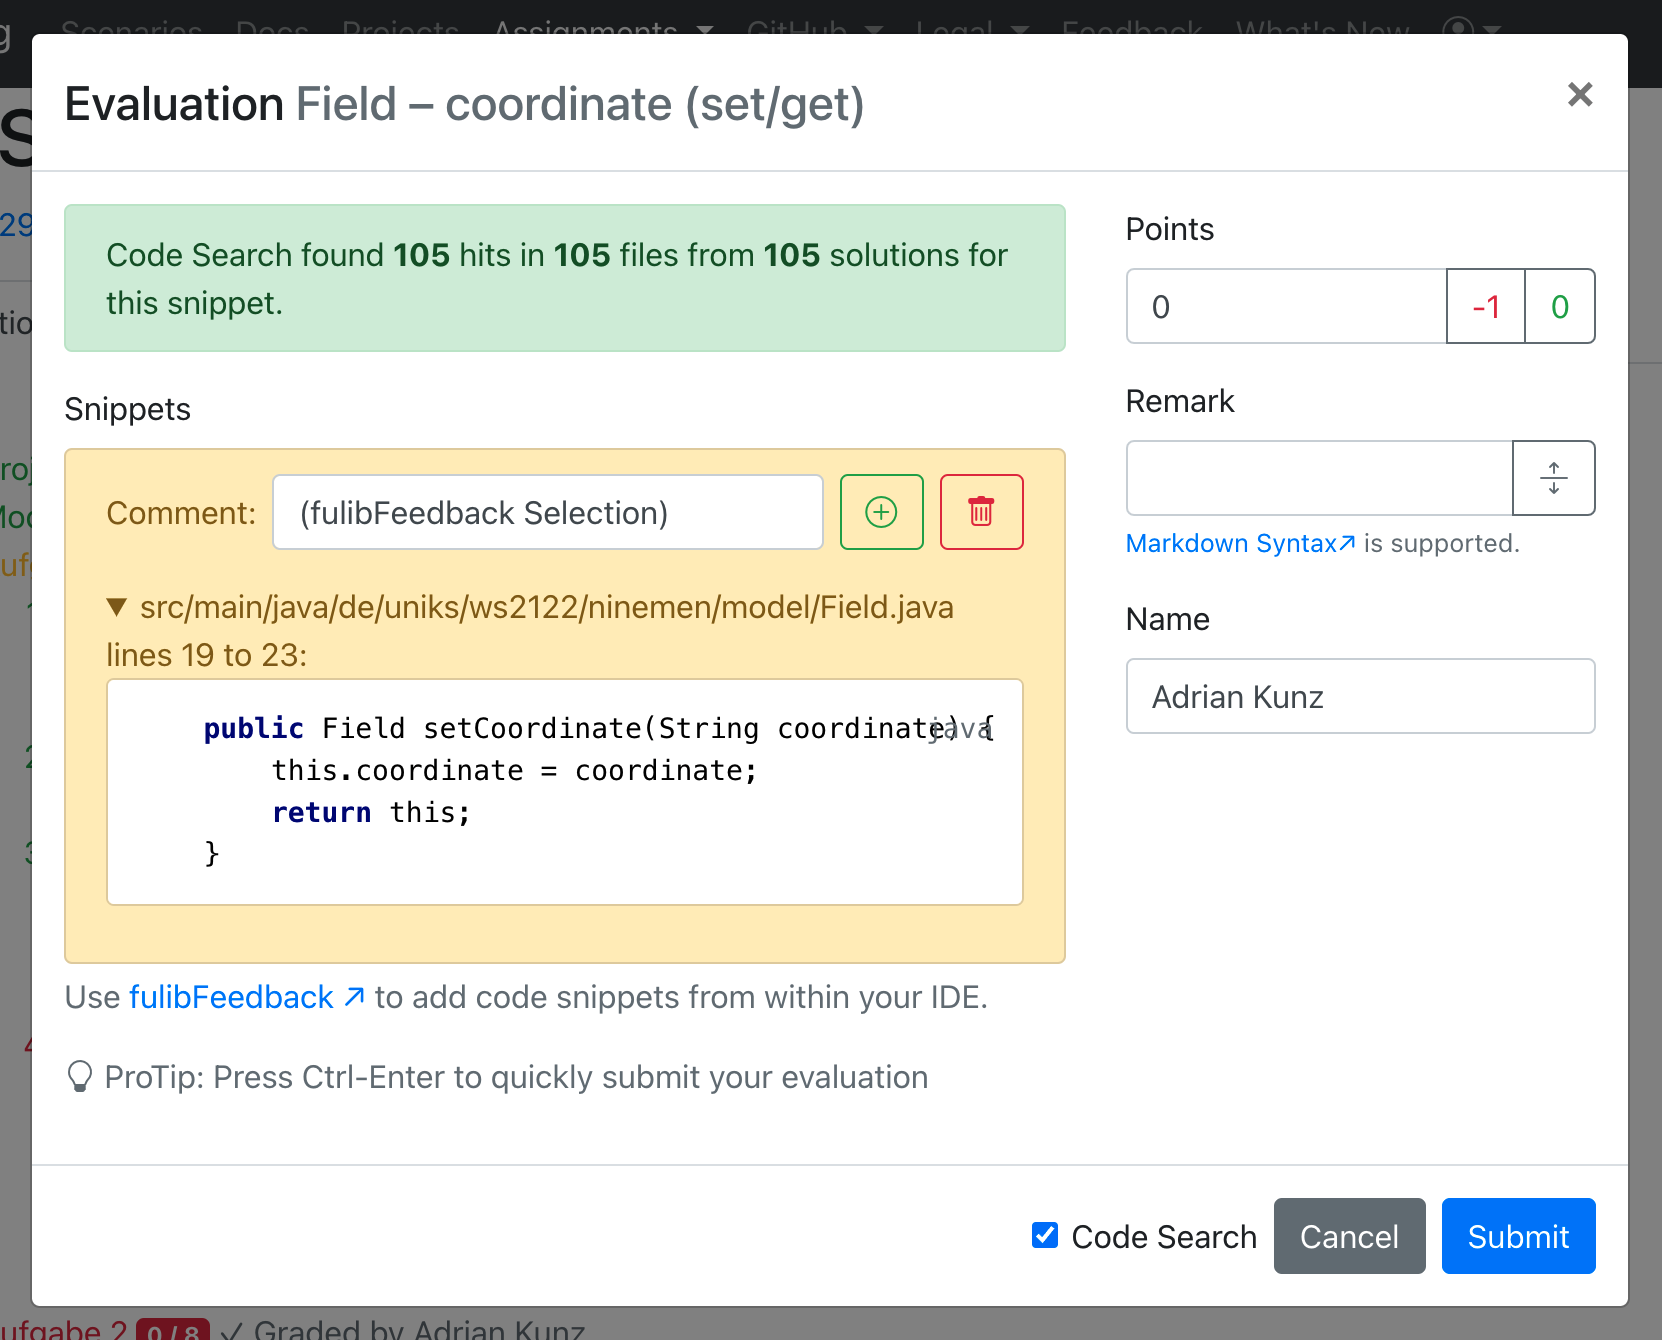
\includegraphics[width=0.8\textwidth]{images/fulibFeedback-snippet-good}
    \caption{Bewertungs-Modalfenster nach Auswahl eines Codeabschnitts}
    \label{fig:fulibFeedback-snippet-good}
\end{figure}

Abbildung~\ref{fig:fulibFeedback-snippet-good} zeigt ein Beispiel, wie sich die Ansicht des Fensters verändert.
Das Formular für die Bewertung wird schmaler und auf der linken Seite erscheint ein neuer Bereich, in dem der Codeabschnitt sowie die Kontextdaten angezeigt werden.
Der Code dient zunächst nur als Vorauswahl und wird erst durch Klick auf den Plus-Button hinzugefügt.
Alternativ kann im Textfeld \textbf{Comment} ein Kommentar für den Codeabschnitt hinterlegt werden.
Dieser unterscheided sich vom Remark insofern, dass er abschnittspezifische Hinweise erlaubt.
Dies ist besonders hilfreich, wenn mehrere Abschnitte zur gleichen Bewertung hinzugefügt werden.

Nach Hinzufügen eines Codeabschnitts kann erneut mit \textbf{Submit} die Bewertung angelegt werden.
Nun kommt der Haken \textbf{Code Search} zum Einsatz.
Ist dieser aktiviert, wird der Codeabschnitt in allen anderen Lösungen mittels Code Search gesucht.
Die Bewertung, insbesondere die Kommentare, Punktzahl und Remark, wird dann auf alle Abgaben übertragen, in denen der Code gefunden wurde.
Dadurch kann abhängig von der Einzigartigkeit des Codes eine Vielzahl von Abgaben in einem Schritt bewertet und Zeit gespart werden.

Bei jeder Auswahl von Code wird Code Search für den diesen durchgeführt.
Dies ergibt eine Liste von Suchergebnissen, aus der drei Metriken ermittelt werden können.
Die Anzahl der \textbf{Solutions} gibt an, wie viele Abgaben den Codeabschnitt enthalten.
In jeder Abgabe können \ac{uU} mehrere Dateien gefundenen werden, die Gesamtanzahl über alle Abgaben ist in \textbf{Files} summiert.
Zuletzt gibt \textbf{Hits} die Anzahl der Suchergebnisse an, die auch mehrfach in einer Datei vorhanden sein können.
Werden diese drei Werte verglichen, kann eine Einschätzung über die Spezifität des Codeabschnitts erfolgen.
Sind alle drei Werte gleich, wie in Abbildung~\ref{fig:fulibFeedback-snippet-good} der Fall ist, kommt der Codeabschnitt in jeder Lösung exakt ein Mal vor.
Das deutet darauf hin, dass er problemlos für die automatische Bewertung mit Code Search verwendet werden kann.

Die Wahl des Codeabschnitts ist mitunter maßgeblich für die Effektivität und Korrektheit von Bewertungen mit Code Search.
Kapitel~\ref{ch:evaluation} untersucht ausführlich anhand einiger realen Beispiele diesen Zusammenhang.
Zunächst werden noch zwei Fälle betrachtet, in denen die Ergebniswerte ungleich sind und zu Problemen führen können.
Die Abbildungen~\ref{fig:fulibFeedback-snippet-bad} und~\ref{fig:fulibFeedback-snippet-worst} zeigen diese Fälle.

\begin{figure}
    \centering
    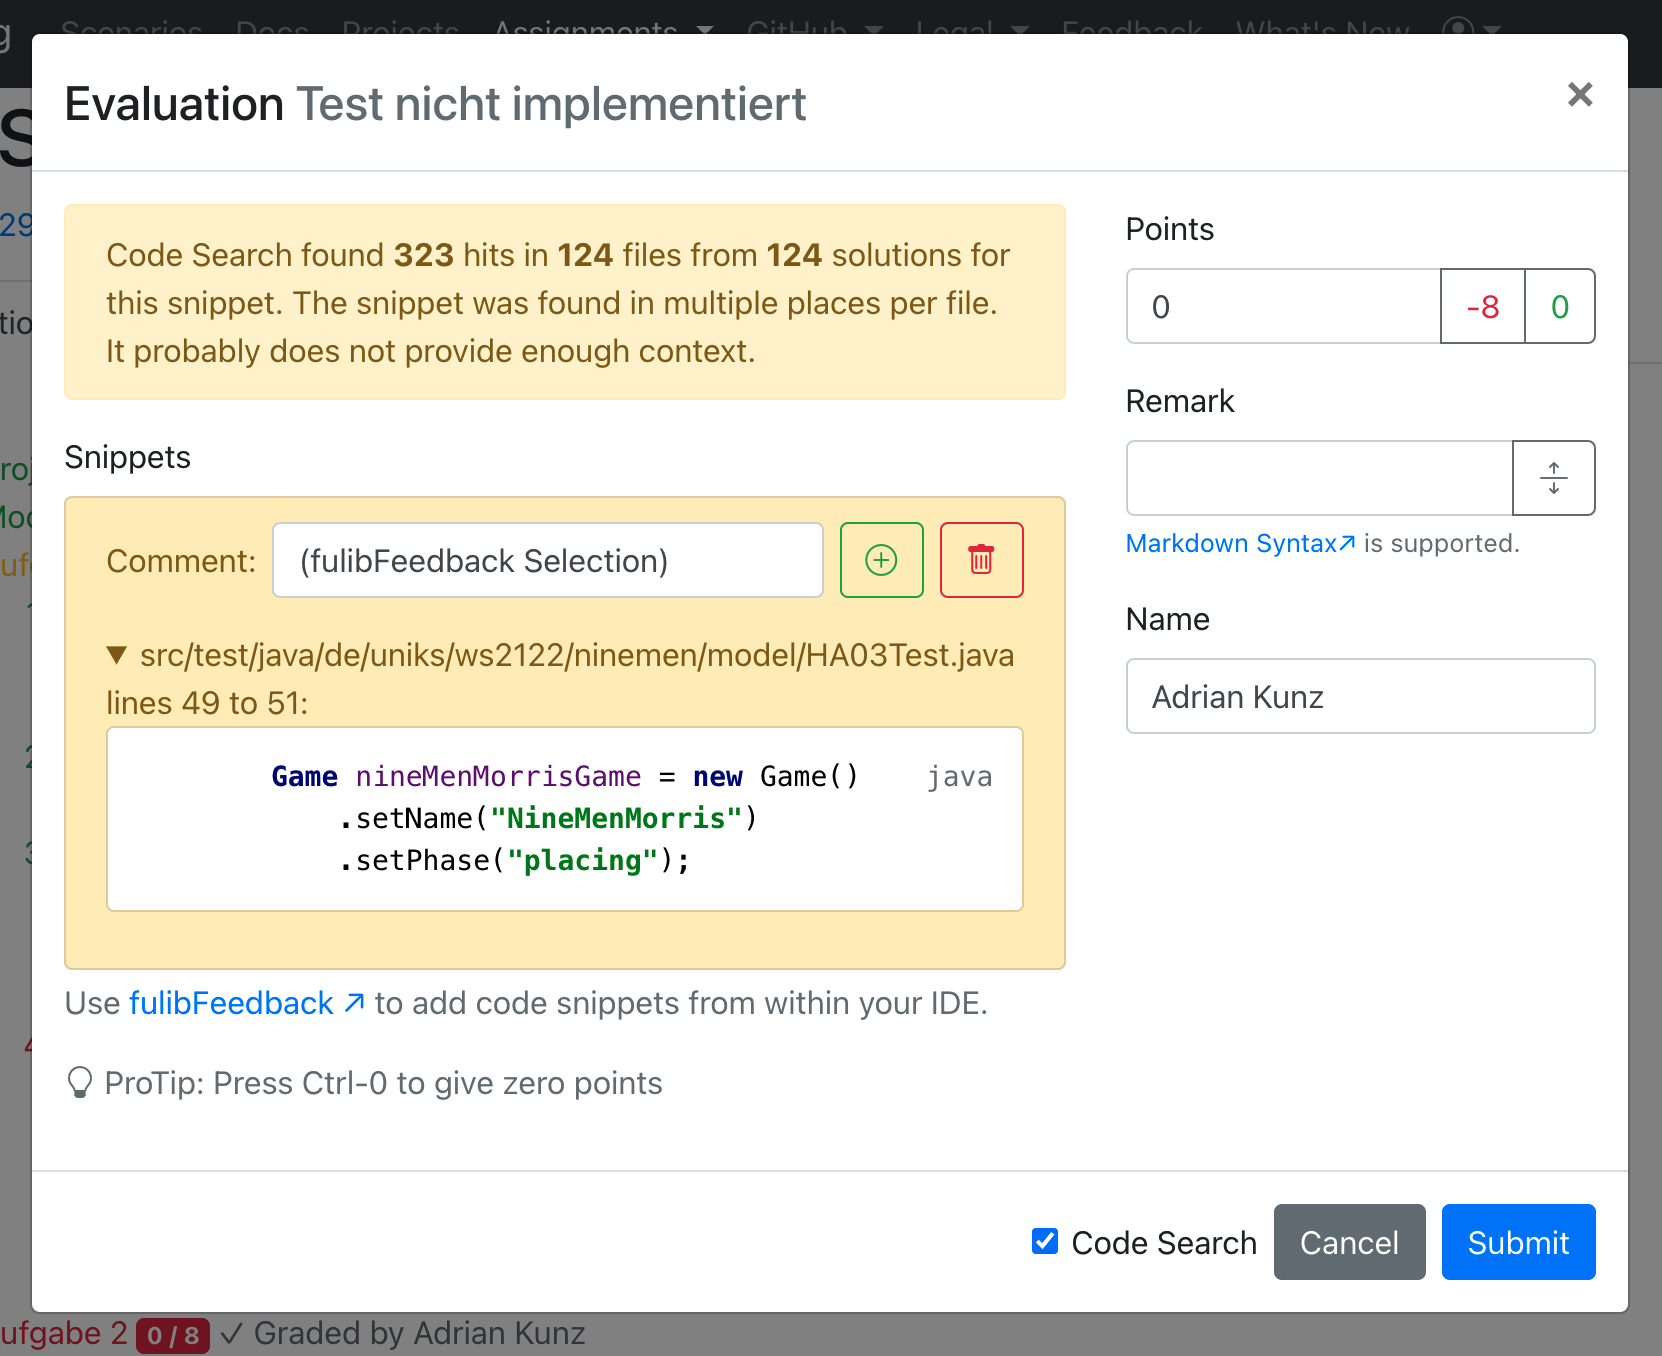
\includegraphics[width=0.8\textwidth]{images/fulibFeedback-snippet-bad}
    \caption{Codeabschnitt mit mehr Suchergebnissen als gefundenen Dateien}
    \label{fig:fulibFeedback-snippet-bad}
\end{figure}

In Abbildung~\ref{fig:fulibFeedback-snippet-bad} wurde eine Codeabschnitt ausgewählt, dessen Suche mehr Ergebnisse als betroffene Dateien, aber in jeder Lösungen nur eine Datei ergeben hat.
Das deutet darauf hin, dass der Code in manchen Lösungen mehrfach in der gleichen Datei vorhanden war.
Bezieht sich die Teilaufgabe beispielsweise auf eine bestimmte Methode, wie in diesem Fall einen Test, kann dies zu unerwünschten Bewertungen führen.
In diesem Beispiel war die Aufgabe, eine neue Testmethode in der vorgegebenen Testklasse \code{HA03Test} hinzuzufügen.
In dieser musste unter anderem ein Datenmodell initialisiert werden.
Der ausgewählte Code in Abbildung~\ref{fig:fulibFeedback-snippet-bad} wurde jedoch in dieser Klasse schon in einer anderen Methode vorgegeben.
Dies ist auch daran ersichtlich, dass nahezu alle Abgaben diesen Code enthalten (124 von 125).
Der ausgewählte Code ist folglich kein sinnvolle Indiz dafür, dass die Aufgabe "Test implementieren" korrekt umgesetzt wurde.
Die gelbe Warnmeldung weist auf diesen Sachverhalt mit der Information hin, dass die Auswahl nicht ausreichend Kontext bietet.
Eine mögliche Lösung ist hier, zusätzlich die voranstehenden Zeilen auszuwählen, die den Kopf der hinzuzufügenden Testmethode enthalten.
Dann wären Suchergebnisse stets eindeutig pro Lösung.

\begin{figure}
    \centering
    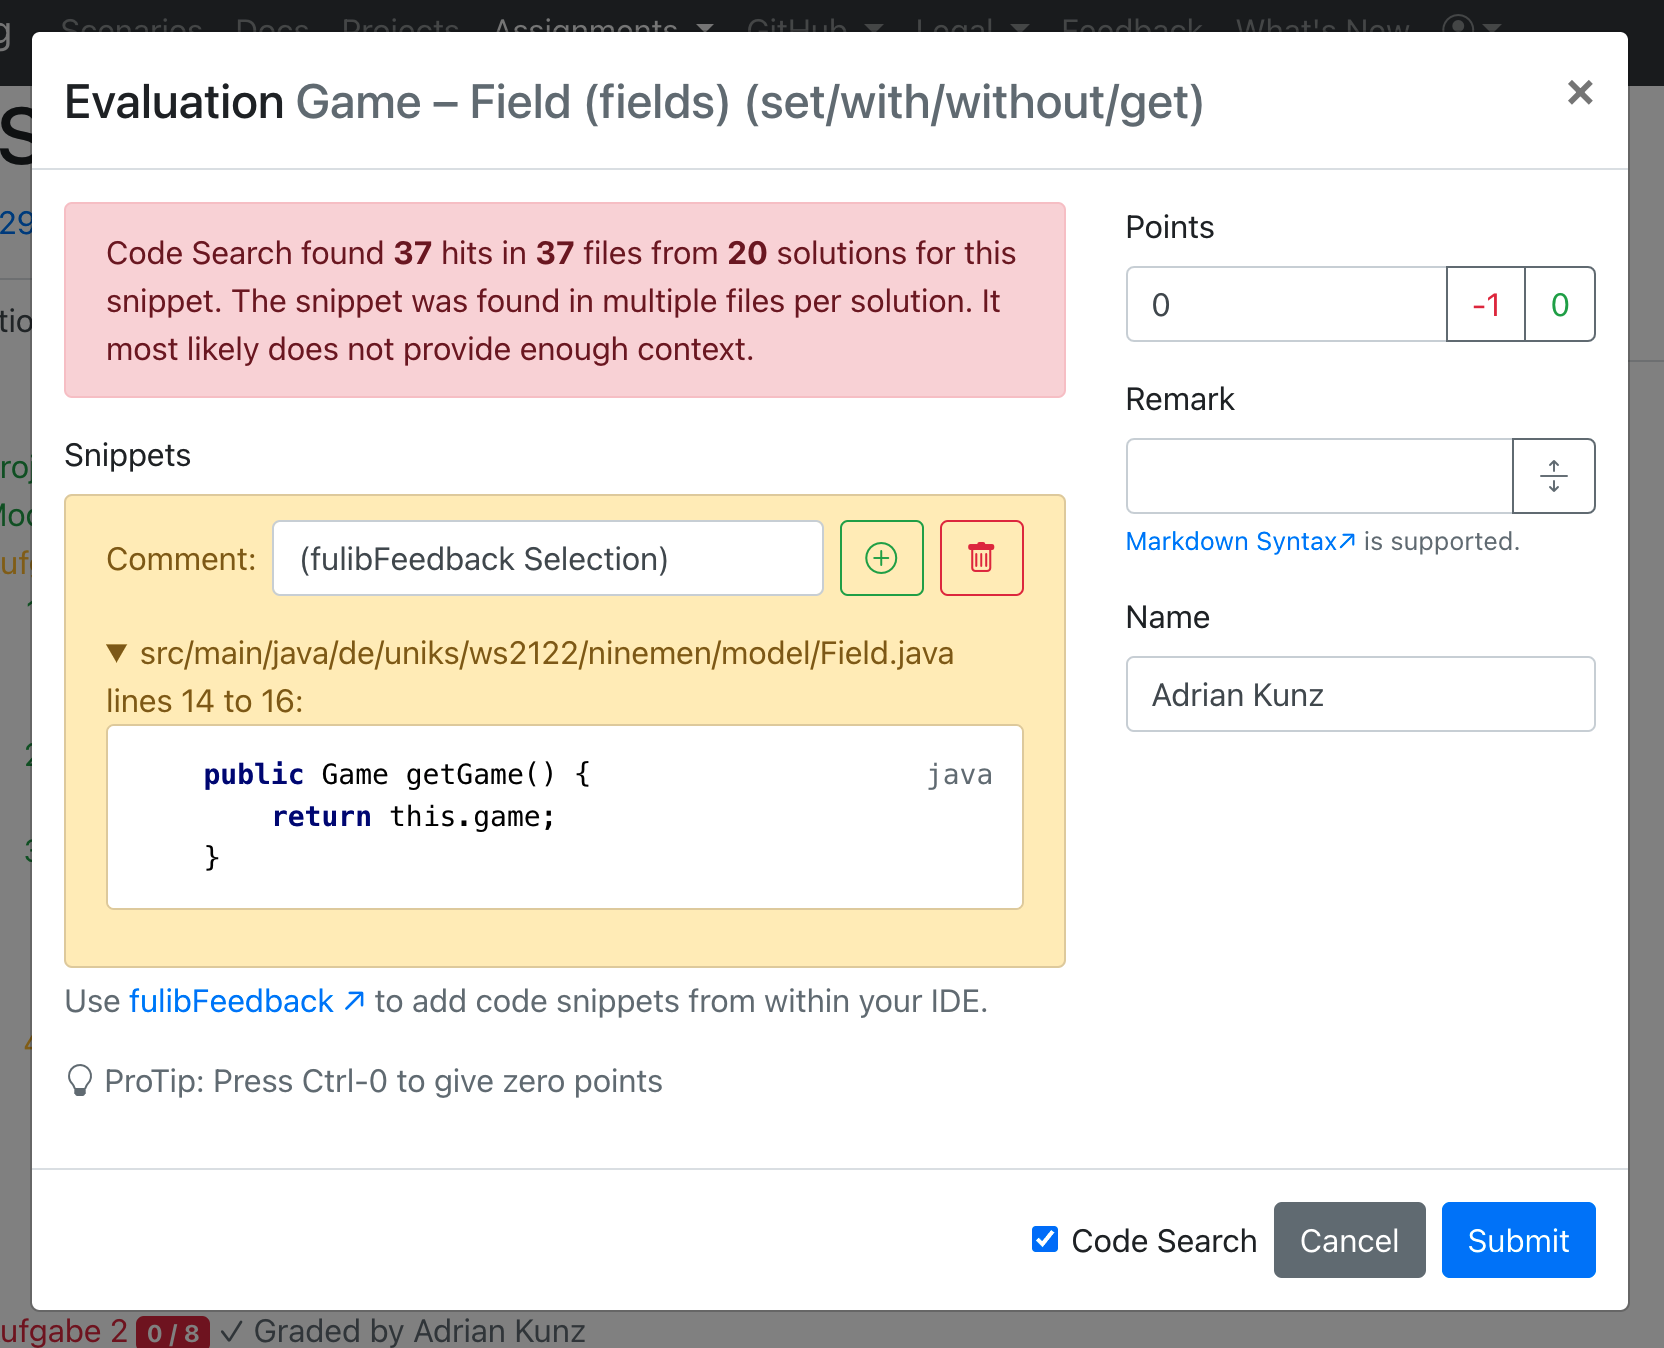
\includegraphics[width=0.8\textwidth]{images/fulibFeedback-snippet-worst}
    \caption{Codeabschnitt mit mehr gefundenen Dateien als Lösungen}
    \label{fig:fulibFeedback-snippet-worst}
\end{figure}

In Abbildung~\ref{fig:fulibFeedback-snippet-worst} gibt es ein ähnliches Problem.
Hier ist jedoch die Anzahl der Dateien mit Suchergebnissen größer als die Anzahl der Lösungen.
Auch dies ist ein Indiz dafür, dass der ausgewählte Code nicht einzigartig ist oder genug Kontext bietet.
In diesem Beispiel wurde ein Getter ausgewählt, der neben \code{Field} auch in anderen Klassen vorkommt.
Hier ist es nicht möglich, mehr Kontext bereitzustellen, da bereits eine ganze Methode ausgewählt wurde.
Stattdessen ist aufgabenspezifisch die Auswahl des Setters sinnvoller, da in diesem Beispiel die korrekte Implementierung von referentieller Integrität gefragt war.

\subsection{Darstellung von Bewertungen}

Bewertungen, bei denen Codeabschnitte hinterlegt wurden, können von fulibFeedback im Editor angezeigt werden.
Dies ist besonders für Studierende nützlich, die nach der Einrichtung der Erweiterungseinstellungen betrachten können, an welchen Stellen im Code zu Punktabzügen geführt haben und welche Teilaufgaben betroffen sind.
Abbildung~\ref{fig:fulibFeedback-negative} zeigen die Markierung im Code sowie den Hilfetext, der beim Hovern über die betroffene Stelle dargestellt wird.

\begin{figure}
    \centering
    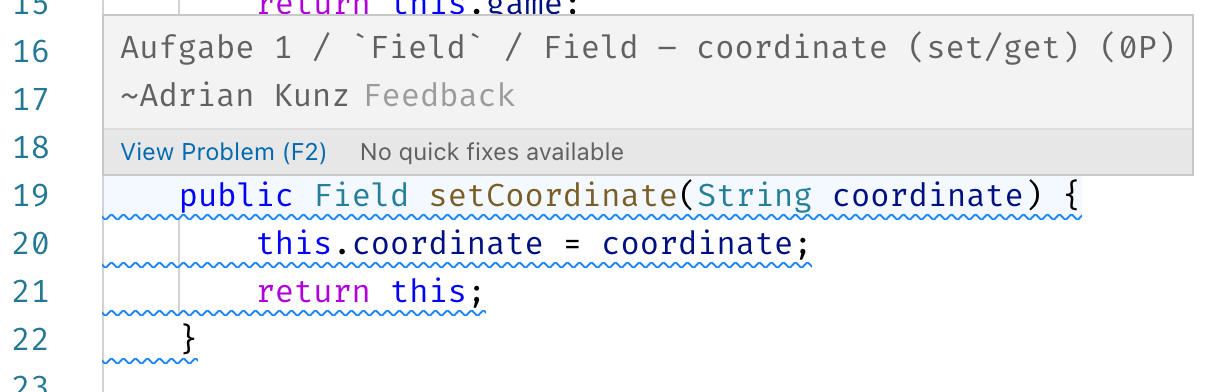
\includegraphics[width=0.83\textwidth]{images/fulibFeedback-positive}
    \caption{Negative Bewertung als Markierung im Code}
    \label{fig:fulibFeedback-negative}
\end{figure}

Abhängig von der vergebenen Punktzahl ändert sich die Farbe der gewellten Linie, welche die Markierung ausmacht.
Wurde die maximale Punktzahl für die Teilaufgabe erreicht ist die Linie blau.
Abzüge oder positive Teilaufgaben mit null Punkten färben die Linie rot wie in Abbildung~\ref{fig:fulibFeedback-negative}.
Teilpunkte werden mit gelber Farbe signalisiert.
Der Hilfetext enthält die Beschreibung der Teilaufgabe (\texttt{Aufgabe 1 / Assoziationen / Game -- Field (fields) \dots}), die vergebene Punktzahl (\texttt{(-1P)}), Remark (\texttt{Rückrichtung nicht gesetzt}) und Kommentar (\texttt{Hier fehlt oldGame.withoutFields(this)}) und den Autor der Bewertung (\texttt{Adrian Kunz}).
Wurden mehrere Codeabschnitte hinterlegt, werden Links angezeigt, die auf andere betroffene Dateien und Zeilen verweisen und den zugehörigen Kommentar angeben (\texttt{Game.java(115, 1): Sehr gut!} und \texttt{Game.java(130, 1): Richtig}).

\subsection{Umsetzung}

\todo{
    VSCode Extension Client:
    Einfacher Client für Language Server.
    Configuration Points für Einstellungen.
    Protocol Handler für Auto-Configure.
    Language Server:
    Selection mit Code Actions.
    Diagnostics.
    Wiederverwendbar für andere IDEs.
}
